%%%%%%%%%%%%%%
%% Run LaTeX on this file several times to get Table of Contents,
%% cross-references, and citations.

%% If you have font problems, you may edit the w-bookps.sty file
%% to customize the font names to match those on your system.

%% w-bksamp.tex. Current Version: Feb 16, 2012
%%%%%%%%%%%%%%%%%%%%%%%%%%%%%%%%%%%%%%%%%%%%%%%%%%%%%%%%%%%%%%%%
%
%  Sample file for
%  Wiley Book Style, Design No.: SD 001B, 7x10
%  Wiley Book Style, Design No.: SD 004B, 6x9
%
%
%  Prepared by Amy Hendrickson, TeXnology Inc.
%  http://www.texnology.com
%%%%%%%%%%%%%%%%%%%%%%%%%%%%%%%%%%%%%%%%%%%%%%%%%%%%%%%%%%%%%%%%

%%%%%%%%%%%%%
% 7x10
%\documentclass{wileySev}

% 6x9
\documentclass{wileySix}

\usepackage{graphicx}
\usepackage{listings}
\usepackage{float}
\usepackage{color}

\definecolor{codegreen}{rgb}{0,0.6,0}
\definecolor{codegray}{rgb}{0.5,0.5,0.5}
\definecolor{codepurple}{rgb}{0.58,0,0.82}
\definecolor{backcolour}{rgb}{0.95,0.95,0.92}

\lstdefinestyle{mystyle}{
    backgroundcolor=\color{backcolour},
    commentstyle=\color{codegreen},
    keywordstyle=\color{magenta},
    numberstyle=\tiny\color{codegray},
    stringstyle=\color{codepurple},
    basicstyle=\footnotesize,
    breakatwhitespace=false,
    breaklines=true,
    captionpos=b,
    keepspaces=true,
    numbers=left,
    numbersep=5pt,
    showspaces=false,
    showstringspaces=false,
    showtabs=false,
    tabsize=2,
    language=sh
}

\lstset{style=mystyle}

%%%%%%%
%% for times math: However, this package disables bold math (!)
%% \mathbf{x} will still work, but you will not have bold math
%% in section heads or chapter titles. If you don't use math
%% in those environments, mathptmx might be a good choice.

% \usepackage{mathptmx}

% For PostScript text
\usepackage{w-bookps}

%%%%%%%%%%%%%%%%%%%%%%%%%%%%%%%%%%%%%%%%%%%%%%%%%%%%%%%%%%%%%%%%
%% Other packages you might want to use:

% for chapter bibliography made with BibTeX
% \usepackage{chapterbib}

% for multiple indices
% \usepackage{multind}

% for answers to problems
% \usepackage{answers}

%%%%%%%%%%%%%%%%%%%%%%%%%%%%%%
%% Change options here if you want:
%%
%% How many levels of section head would you like numbered?
%% 0= no section numbers, 1= section, 2= subsection, 3= subsubsection
%%==>>
\setcounter{secnumdepth}{3}

%% How many levels of section head would you like to appear in the
%% Table of Contents?
%% 0= chapter titles, 1= section titles, 2= subsection titles,
%% 3= subsubsection titles.
%%==>>
\setcounter{tocdepth}{2}

%% Cropmarks? good for final page makeup
%% \docropmarks

%%%%%%%%%%%%%%%%%%%%%%%%%%%%%%
%
% DRAFT
%
% Uncomment to get double spacing between lines, current date and time
% printed at bottom of page.
% \draft
% (If you want to keep tables from becoming double spaced also uncomment
% this):
% \renewcommand{\arraystretch}{0.6}
%%%%%%%%%%%%%%%%%%%%%%%%%%%%%%

%%%%%%% Demo of section head containing sample macro:
%% To get a macro to expand correctly in a section head, with upper and
%% lower case math, put the definition and set the box
%% before \begin{document}, so that when it appears in the
%% table of contents it will also work:

\newcommand{\VT}[1]{\ensuremath{{V_{T#1}}}}

%% use a box to expand the macro before we put it into the section head:

\newbox\sectsavebox
\setbox\sectsavebox=\hbox{\boldmath\VT{xyz}}

%%%%%%%%%%%%%%%%% End Demo


\begin{document}


\booktitle{Cerdas Menguasai Python}
\subtitle{Dalam 24 Jam}

\authors{Rolly M. Awangga\\
\affil{Informatics Research Center}
%Floyd J. Fowler, Jr.\\
%\affil{University of New Mexico}
}

\offprintinfo{Cerdas Menguasai Python, First Edition}{Rolly M. Awangga}

%% Can use \\ if title, and edition are too wide, ie,
%% \offprintinfo{Survey Methodology,\\ Second Edition}{Robert M. Groves}

%%%%%%%%%%%%%%%%%%%%%%%%%%%%%%
%%
\halftitlepage

%\titlepage


\begin{copyrightpage}{2019}
%Survey Methodology / Robert M. Groves . . . [et al.].
%\       p. cm.---(Wiley series in survey methodology)
%\    ``Wiley-Interscience."
%\    Includes bibliographical references and index.
%\    ISBN 0-471-48348-6 (pbk.)
%\    1. Surveys---Methodology.  2. Social 
%\  sciences---Research---Statistical methods.  I. Groves, Robert M.  II. %
%Series.\\
%
%HA31.2.S873 2007
%001.4'33---dc22                                             2004044064
\end{copyrightpage}

\dedication{`Jika Kamu tidak dapat menahan lelahnya belajar,
Maka kamu harus sanggup menahan perihnya Kebodohan.'
~Imam Syafi'i~}

\begin{contributors}
\name{Rolly Maulana Awangga,} Informatics Research Center., Politeknik Pos Indonesia, Bandung,
Indonesia



\end{contributors}

\contentsinbrief
\tableofcontents
\listoffigures
\listoftables
\lstlistoflistings


\begin{foreword}
Sepatah kata dari Kaprodi, Kabag Kemahasiswaan dan Mahasiswa
\end{foreword}

\begin{preface}
Buku ini diciptakan bagi yang awam dengan flask sekalipun.

\prefaceauthor{R. M. Awangga}
\where{Bandung, Jawa Barat\\
Februari, 2019}
\end{preface}


\begin{acknowledgments}
Terima kasih atas semua masukan dari para mahasiswa agar bisa membuat buku ini 
lebih baik dan lebih mudah dimengerti.

Terima kasih ini juga ditujukan khusus untuk team IRC yang 
telah fokus untuk belajar dan memahami bagaimana buku ini mendampingi proses 
Intership.
\authorinitials{R. M. A.}
\end{acknowledgments}

\begin{acronyms}
\acro{ACGIH}{American Conference of Governmental Industrial Hygienists}
\acro{AEC}{Atomic Energy Commission}
\acro{OSHA}{Occupational Health and Safety Commission}
\acro{SAMA}{Scientific Apparatus Makers Association}
\end{acronyms}

\begin{glossary}
\term{git}Merupakan manajemen sumber kode yang dibuat oleh linus torvald.

\term{bash}Merupakan bahasa sistem operasi berbasiskan *NIX.

\term{linux}Sistem operasi berbasis sumber kode terbuka yang dibuat oleh Linus Torvald
\end{glossary}

\begin{symbols}
\term{A}Amplitude

\term{\hbox{\&}}Propositional logic symbol 

\term{a}Filter Coefficient

\bigskip

\term{\mathcal{B}}Number of Beats
\end{symbols}

\begin{introduction}

%% optional, but if you want to list author:

\introauthor{Rolly Maulana Awangga, S.T., M.T.}
{Informatics Research Center\\
Bandung, Jawa Barat, Indonesia}

Pada era disruptif  \index{disruptif}\index{disruptif!modern} 
saat ini. git merupakan sebuah kebutuhan dalam sebuah organisasi pengembangan perangkat lunak.
Buku ini diharapkan bisa menjadi penghantar para programmer, analis, IT Operation dan Project Manajer.
Dalam melakukan implementasi git pada diri dan organisasinya.

Rumusnya cuman sebagai contoh aja biar keren\cite{awangga2018sampeu}.

\begin{equation}
ABC {\cal DEF} \alpha\beta\Gamma\Delta\sum^{abc}_{def}
\end{equation}

\end{introduction}

%%%%%%%%%%%%%%%%%%Isi Buku_
%TEORI
%\chapter{Judul Bagian Pertama}
%\section{Arjun Yuda Firwanda}
\subsection{Soal 1}
Isi jawaban soal ke-1

Kalau mau dibikin paragrap \textbf{cukup enter aja}, tidak usah pakai \verb|par| dsb

%\subsection{Soal 2}
%Isi jawaban soal ke-2

%\subsection{Soal 3}
%Isi jawaban soal ke-3

\section{Dwi Yulianingsih}
\subsection{Soal 1}
Isi jawaban soal ke-1

Kalau mau dibikin paragrap \textbf{cukup enter aja}, tidak usah pakai \verb|par| dsb

%\subsection{Soal 2}
%Isi jawaban soal ke-2

%\subsection{Soal 3}
%Isi jawaban soal ke-3

\section{Harun Ar-Rasyid}
\subsection{Soal 1}
Isi jawaban soal ke-1

Kalau mau dibikin paragrap \textbf{cukup enter aja}, tidak usah pakai \verb|par| dsb

%\subsection{Soal 2}
%Isi jawaban soal ke-2

%\subsection{Soal 3}
%Isi jawaban soal ke-3

\section{Sri Rahayu}
\subsection{Soal 1}
Isi jawaban soal ke-1

Kalau mau dibikin paragrap \textbf{cukup enter aja}, tidak usah pakai \verb|par| dsb

%\subsection{Soal 2}
%Isi jawaban soal ke-2

%\subsection{Soal 3}
%Isi jawaban soal ke-3

\section{Doli Jonviter}
\subsection{Soal 1}
Isi jawaban soal ke-1

Kalau mau dibikin paragrap \textbf{cukup enter aja}, tidak usah pakai \verb|par| dsb

%\subsection{Soal 2}
%Isi jawaban soal ke-2

%\subsection{Soal 3}
%Isi jawaban soal ke-3

\section{Rahmatul Ridha}
\subsection{Soal 1}
Isi jawaban soal ke-1

Kalau mau dibikin paragrap \textbf{cukup enter aja}, tidak usah pakai \verb|par| dsb

%\subsection{Soal 2}
%Isi jawaban soal ke-2

%\subsection{Soal 3}
%Isi jawaban soal ke-3

\section{Tomy Prawoto}
\subsection{Soal 1}
Isi jawaban soal ke-1

Kalau mau dibikin paragrap \textbf{cukup enter aja}, tidak usah pakai \verb|par| dsb

%\subsection{Soal 2}
%Isi jawaban soal ke-2

%\subsection{Soal 3}
%Isi jawaban soal ke-3

%PRAKTEK
%\chapter{Judul Bagian Pertama}
%\section{Arjun Yuda Firwanda}
\subsection{Soal 1}
Isi jawaban soal ke-1

Kalau mau dibikin paragrap \textbf{cukup enter aja}, tidak usah pakai \verb|par| dsb

%\subsection{Soal 2}
%Isi jawaban soal ke-2

%\subsection{Soal 3}
%Isi jawaban soal ke-3

\section{Dwi Yulianingsih}
\subsection{Soal 1}
Isi jawaban soal ke-1

Kalau mau dibikin paragrap \textbf{cukup enter aja}, tidak usah pakai \verb|par| dsb

%\subsection{Soal 2}
%Isi jawaban soal ke-2

%\subsection{Soal 3}
%Isi jawaban soal ke-3

\section{Harun Ar-Rasyid}
\subsection{Soal 1}
Isi jawaban soal ke-1

Kalau mau dibikin paragrap \textbf{cukup enter aja}, tidak usah pakai \verb|par| dsb

%\subsection{Soal 2}
%Isi jawaban soal ke-2

%\subsection{Soal 3}
%Isi jawaban soal ke-3

\section{Sri Rahayu}
\subsection{Soal 1}
Isi jawaban soal ke-1

Kalau mau dibikin paragrap \textbf{cukup enter aja}, tidak usah pakai \verb|par| dsb

%\subsection{Soal 2}
%Isi jawaban soal ke-2

%\subsection{Soal 3}
%Isi jawaban soal ke-3

\section{Doli Jonviter}
\subsection{Soal 1}
Isi jawaban soal ke-1

Kalau mau dibikin paragrap \textbf{cukup enter aja}, tidak usah pakai \verb|par| dsb

%\subsection{Soal 2}
%Isi jawaban soal ke-2

%\subsection{Soal 3}
%Isi jawaban soal ke-3

\section{Rahmatul Ridha}
\subsection{Soal 1}
Isi jawaban soal ke-1

Kalau mau dibikin paragrap \textbf{cukup enter aja}, tidak usah pakai \verb|par| dsb

%\subsection{Soal 2}
%Isi jawaban soal ke-2

%\subsection{Soal 3}
%Isi jawaban soal ke-3

\section{Tomy Prawoto}
\subsection{Soal 1}
Isi jawaban soal ke-1

Kalau mau dibikin paragrap \textbf{cukup enter aja}, tidak usah pakai \verb|par| dsb

%\subsection{Soal 2}
%Isi jawaban soal ke-2

%\subsection{Soal 3}
%Isi jawaban soal ke-3


%TEORI
%\chapter{Judul Bagian Pertama}
%\section{Arjun Yuda Firwanda}
\subsection{Soal 1}
Isi jawaban soal ke-1

Kalau mau dibikin paragrap \textbf{cukup enter aja}, tidak usah pakai \verb|par| dsb

%\subsection{Soal 2}
%Isi jawaban soal ke-2

%\subsection{Soal 3}
%Isi jawaban soal ke-3

\section{Dwi Yulianingsih}
\subsection{Soal 1}
Isi jawaban soal ke-1

Kalau mau dibikin paragrap \textbf{cukup enter aja}, tidak usah pakai \verb|par| dsb

%\subsection{Soal 2}
%Isi jawaban soal ke-2

%\subsection{Soal 3}
%Isi jawaban soal ke-3

\section{Harun Ar-Rasyid}
\subsection{Soal 1}
Isi jawaban soal ke-1

Kalau mau dibikin paragrap \textbf{cukup enter aja}, tidak usah pakai \verb|par| dsb

%\subsection{Soal 2}
%Isi jawaban soal ke-2

%\subsection{Soal 3}
%Isi jawaban soal ke-3

\section{Sri Rahayu}
\subsection{Soal 1}
Isi jawaban soal ke-1

Kalau mau dibikin paragrap \textbf{cukup enter aja}, tidak usah pakai \verb|par| dsb

%\subsection{Soal 2}
%Isi jawaban soal ke-2

%\subsection{Soal 3}
%Isi jawaban soal ke-3

\section{Doli Jonviter}
\subsection{Soal 1}
Isi jawaban soal ke-1

Kalau mau dibikin paragrap \textbf{cukup enter aja}, tidak usah pakai \verb|par| dsb

%\subsection{Soal 2}
%Isi jawaban soal ke-2

%\subsection{Soal 3}
%Isi jawaban soal ke-3

\section{Rahmatul Ridha}
\subsection{Soal 1}
Isi jawaban soal ke-1

Kalau mau dibikin paragrap \textbf{cukup enter aja}, tidak usah pakai \verb|par| dsb

%\subsection{Soal 2}
%Isi jawaban soal ke-2

%\subsection{Soal 3}
%Isi jawaban soal ke-3

\section{Tomy Prawoto}
\subsection{Soal 1}
Isi jawaban soal ke-1

Kalau mau dibikin paragrap \textbf{cukup enter aja}, tidak usah pakai \verb|par| dsb

%\subsection{Soal 2}
%Isi jawaban soal ke-2

%\subsection{Soal 3}
%Isi jawaban soal ke-3

%PRAKTEK
%\chapter{Judul Bagian Pertama}
%\section{Arjun Yuda Firwanda}
\subsection{Soal 1}
Isi jawaban soal ke-1

Kalau mau dibikin paragrap \textbf{cukup enter aja}, tidak usah pakai \verb|par| dsb

%\subsection{Soal 2}
%Isi jawaban soal ke-2

%\subsection{Soal 3}
%Isi jawaban soal ke-3

\section{Dwi Yulianingsih}
\subsection{Soal 1}
Isi jawaban soal ke-1

Kalau mau dibikin paragrap \textbf{cukup enter aja}, tidak usah pakai \verb|par| dsb

%\subsection{Soal 2}
%Isi jawaban soal ke-2

%\subsection{Soal 3}
%Isi jawaban soal ke-3

\section{Harun Ar-Rasyid}
\subsection{Soal 1}
Isi jawaban soal ke-1

Kalau mau dibikin paragrap \textbf{cukup enter aja}, tidak usah pakai \verb|par| dsb

%\subsection{Soal 2}
%Isi jawaban soal ke-2

%\subsection{Soal 3}
%Isi jawaban soal ke-3

\section{Sri Rahayu}
\subsection{Soal 1}
Isi jawaban soal ke-1

Kalau mau dibikin paragrap \textbf{cukup enter aja}, tidak usah pakai \verb|par| dsb

%\subsection{Soal 2}
%Isi jawaban soal ke-2

%\subsection{Soal 3}
%Isi jawaban soal ke-3

\section{Doli Jonviter}
\subsection{Soal 1}
Isi jawaban soal ke-1

Kalau mau dibikin paragrap \textbf{cukup enter aja}, tidak usah pakai \verb|par| dsb

%\subsection{Soal 2}
%Isi jawaban soal ke-2

%\subsection{Soal 3}
%Isi jawaban soal ke-3

\section{Rahmatul Ridha}
\subsection{Soal 1}
Isi jawaban soal ke-1

Kalau mau dibikin paragrap \textbf{cukup enter aja}, tidak usah pakai \verb|par| dsb

%\subsection{Soal 2}
%Isi jawaban soal ke-2

%\subsection{Soal 3}
%Isi jawaban soal ke-3

\section{Tomy Prawoto}
\subsection{Soal 1}
Isi jawaban soal ke-1

Kalau mau dibikin paragrap \textbf{cukup enter aja}, tidak usah pakai \verb|par| dsb

%\subsection{Soal 2}
%Isi jawaban soal ke-2

%\subsection{Soal 3}
%Isi jawaban soal ke-3


%TEORI
%\chapter{Judul Bagian Pertama}
%\section{Arjun Yuda Firwanda}
\subsection{Soal 1}
Isi jawaban soal ke-1

Kalau mau dibikin paragrap \textbf{cukup enter aja}, tidak usah pakai \verb|par| dsb

%\subsection{Soal 2}
%Isi jawaban soal ke-2

%\subsection{Soal 3}
%Isi jawaban soal ke-3

\section{Dwi Yulianingsih}
\subsection{Soal 1}
Isi jawaban soal ke-1

Kalau mau dibikin paragrap \textbf{cukup enter aja}, tidak usah pakai \verb|par| dsb

%\subsection{Soal 2}
%Isi jawaban soal ke-2

%\subsection{Soal 3}
%Isi jawaban soal ke-3

\section{Harun Ar-Rasyid}
\subsection{Soal 1}
Isi jawaban soal ke-1

Kalau mau dibikin paragrap \textbf{cukup enter aja}, tidak usah pakai \verb|par| dsb

%\subsection{Soal 2}
%Isi jawaban soal ke-2

%\subsection{Soal 3}
%Isi jawaban soal ke-3

\section{Sri Rahayu}
\subsection{Soal 1}
Isi jawaban soal ke-1

Kalau mau dibikin paragrap \textbf{cukup enter aja}, tidak usah pakai \verb|par| dsb

%\subsection{Soal 2}
%Isi jawaban soal ke-2

%\subsection{Soal 3}
%Isi jawaban soal ke-3

\section{Doli Jonviter}
\subsection{Soal 1}
Isi jawaban soal ke-1

Kalau mau dibikin paragrap \textbf{cukup enter aja}, tidak usah pakai \verb|par| dsb

%\subsection{Soal 2}
%Isi jawaban soal ke-2

%\subsection{Soal 3}
%Isi jawaban soal ke-3

\section{Rahmatul Ridha}
\subsection{Soal 1}
Isi jawaban soal ke-1

Kalau mau dibikin paragrap \textbf{cukup enter aja}, tidak usah pakai \verb|par| dsb

%\subsection{Soal 2}
%Isi jawaban soal ke-2

%\subsection{Soal 3}
%Isi jawaban soal ke-3

\section{Tomy Prawoto}
\subsection{Soal 1}
Isi jawaban soal ke-1

Kalau mau dibikin paragrap \textbf{cukup enter aja}, tidak usah pakai \verb|par| dsb

%\subsection{Soal 2}
%Isi jawaban soal ke-2

%\subsection{Soal 3}
%Isi jawaban soal ke-3

%PRAKTEK
%\chapter{Judul Bagian Pertama}
%\section{Arjun Yuda Firwanda}
\subsection{Soal 1}
Isi jawaban soal ke-1

Kalau mau dibikin paragrap \textbf{cukup enter aja}, tidak usah pakai \verb|par| dsb

%\subsection{Soal 2}
%Isi jawaban soal ke-2

%\subsection{Soal 3}
%Isi jawaban soal ke-3

\section{Dwi Yulianingsih}
\subsection{Soal 1}
Isi jawaban soal ke-1

Kalau mau dibikin paragrap \textbf{cukup enter aja}, tidak usah pakai \verb|par| dsb

%\subsection{Soal 2}
%Isi jawaban soal ke-2

%\subsection{Soal 3}
%Isi jawaban soal ke-3

\section{Harun Ar-Rasyid}
\subsection{Soal 1}
Isi jawaban soal ke-1

Kalau mau dibikin paragrap \textbf{cukup enter aja}, tidak usah pakai \verb|par| dsb

%\subsection{Soal 2}
%Isi jawaban soal ke-2

%\subsection{Soal 3}
%Isi jawaban soal ke-3

\section{Sri Rahayu}
\subsection{Soal 1}
Isi jawaban soal ke-1

Kalau mau dibikin paragrap \textbf{cukup enter aja}, tidak usah pakai \verb|par| dsb

%\subsection{Soal 2}
%Isi jawaban soal ke-2

%\subsection{Soal 3}
%Isi jawaban soal ke-3

\section{Doli Jonviter}
\subsection{Soal 1}
Isi jawaban soal ke-1

Kalau mau dibikin paragrap \textbf{cukup enter aja}, tidak usah pakai \verb|par| dsb

%\subsection{Soal 2}
%Isi jawaban soal ke-2

%\subsection{Soal 3}
%Isi jawaban soal ke-3

\section{Rahmatul Ridha}
\subsection{Soal 1}
Isi jawaban soal ke-1

Kalau mau dibikin paragrap \textbf{cukup enter aja}, tidak usah pakai \verb|par| dsb

%\subsection{Soal 2}
%Isi jawaban soal ke-2

%\subsection{Soal 3}
%Isi jawaban soal ke-3

\section{Tomy Prawoto}
\subsection{Soal 1}
Isi jawaban soal ke-1

Kalau mau dibikin paragrap \textbf{cukup enter aja}, tidak usah pakai \verb|par| dsb

%\subsection{Soal 2}
%Isi jawaban soal ke-2

%\subsection{Soal 3}
%Isi jawaban soal ke-3


%TEORI
%\chapter{Library CSV dan Pandas}
%\section{Evietania Charis Sujadi}
\subsection{Fungsi Csv}
Fungsi csv yaitu memudahkan user dalam melakukan input data karena pada csv input data ataupun import data dalam skala besar dapat dilakukan dengan cara yang sederhana.
\subsection{Sejarah Csv}
Dari rilis pertama, Excel menggunakan format file biner yang disebut Binary Interchange File Format (BIFF) sebagai format file utamanya. Ini berubah ketika Microsoft merilis Office System 2007 yang memperkenalkan Office Open XML sebagai format file utamanya. Office Open XML adalah file kontainer berbasis XML yang mirip dengan XML Spreadsheets (XMLSS), yang diperkenalkan di Excel 2002. File versi XML tidak bisa menyimpan makro VBA. Meskipun mendukung format XML baru, Excel 2007 masih mendukung format lama yang masih berbasis BIFF tradisional. Selain itu Microsoft Excel juga mendukung format Comma Separated Values (CSV), DBase File (DBF), SYMbolic LinK (SYLK), Format Interchange Data (DIF) dan banyak format lainnya, termasuk format lembar kerja 1-2 Lotus - 3 (WKS, WK1, WK2, dll.) Dan Quattro Pro.
\lstinputlisting[firstline=7, lastline=20]{src/4/1174051/teori/gatau.py}
\subsection{Aplikasi yang dapat menghasilkan csv}
\begin{itemize}
\item Texteditor
Seperti notepad++,visual studio code,atom,sublime dan lain sebagainya
\item Program Spreadsheet
  Seperti excell,google spreadshare,LibreOfficecalc
 \end{itemize}
\subsection{Jelaskan bagaimana cara menulis dan membaca file csv di excel atau spreadsheet}
Caranya sangat mudah yaitu:
 Untuk menulisnya untuk yang paling atas itu kita buat headernya,untuk mepermudah membedakan datanya,dan untuk baris kedua dan seterusnya itu untuk data itu sendiri.Setelah di buat kalian save as kemudian pilih format CSV.Untuk membukan cukup di double clik file tersebut
\subsection{Jelaskan sejarah library csv}
CSV muncul untuk memudahkan data science dan analis karena dinilai terdapat banyak kemudahan yang didapat. CSV dapat dimaksimalkan jika dipaduka dengan python karena python adalah bahasa pemrograman yang support ke banyak library termasuk csv. Maka karena itulah perpaduan python dan csv seringkali digunakan oleh perusahaan-perushaan besar dalam mengolah datanya.
\subsection{Jelaskan sejarah library pandas}
Pandas merupakan tool yang dapat digunakan sebagai alat analisis data dan struktur untuk bahasa pemrograman Python. Pandas dapat mengolah data dengan mudah, salah satu fitur yang ada dalam pandas adalah Dataframe. Fitur dataframe dapat membaca sebuah file dan menjadikannya tabble, juga dapat mengolah suatu data dengan menggunakan operasi seperti join, group by dan teknik lainnya yang terdapat pada SQL. Dalam hal ini pandas tidak jauh beda dengan csv yaitu memiliki keunggulan dalam pengolahan data-data besar dan dapat disupport dengan baik dengan python walaupun mengimport data dalam jumlah banyak.
\subsection{Fungsi-fungsi Library CSV}
Dalam library csv terdapat dua fungsi yaiut fungsi membaca file dan menulis file csv.
Library csv mempunyai keunggulan dibandingkan format data lainnya adalah soal kompatibilitas. File csv dapat digunakan, diolah, diekspor/impor, dan dimodifikasi menggunakan berbagai macam perangkat lunak dan bahasa pemrograman. Pada library csv mempunyai fungsi import dan eksport data yang baik dan bisa digunakan dalam jumlah besar.
\subsection{Fungsi-fungsi library Pandas}
Pandas pun memiliki fungsi yang sama yaitu menulis dan membaca file. pandas menyediakan beragam fungsi operasi untuk mengolah data. Contoh jika menggunakan series bisa mencari nilai max, min, dan mean secara langsung, bahkan juga bisa melakukan operasi perpangkatan pada nilai Series secara langsung.
Pandas dapat mengolah suatu data dan mengolahnya seperti join, distinct, group by, agregasi, dan teknik seperti pada SQL. Hanya saja dilakukan pada tabel yang dimuat dari file ke RAM.
\subsection{Bukti Plagiarisme}
\begin{figure}[h]
	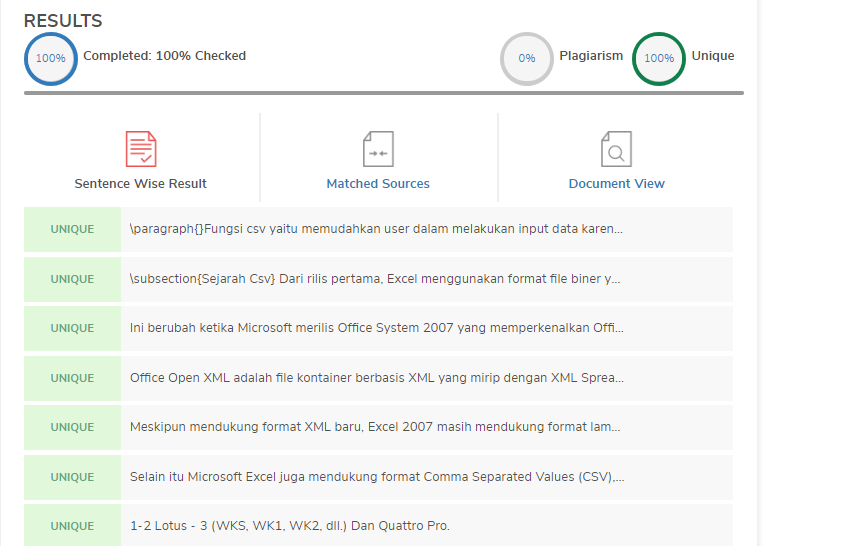
\includegraphics[width=10cm]{figures/4/1174051/teori/nih.png}
	\centering
\end{figure}
\section{Dwi Yulianingsih}
\subsection{Soal 1}
Isi jawaban soal ke-1

Kalau mau dibikin paragrap \textbf{cukup enter aja}, tidak usah pakai \verb|par| dsb

%\subsection{Soal 2}
%Isi jawaban soal ke-2

%\subsection{Soal 3}
%Isi jawaban soal ke-3

\section{Harun Ar-Rasyid}
\subsection{Soal 1}
Isi jawaban soal ke-1

Kalau mau dibikin paragrap \textbf{cukup enter aja}, tidak usah pakai \verb|par| dsb

%\subsection{Soal 2}
%Isi jawaban soal ke-2

%\subsection{Soal 3}
%Isi jawaban soal ke-3

\section{Sri Rahayu}
\subsection{Soal 1}
Isi jawaban soal ke-1

Kalau mau dibikin paragrap \textbf{cukup enter aja}, tidak usah pakai \verb|par| dsb

%\subsection{Soal 2}
%Isi jawaban soal ke-2

%\subsection{Soal 3}
%Isi jawaban soal ke-3

\section{Doli Jonviter}
\subsection{Soal 1}
Isi jawaban soal ke-1

Kalau mau dibikin paragrap \textbf{cukup enter aja}, tidak usah pakai \verb|par| dsb

%\subsection{Soal 2}
%Isi jawaban soal ke-2

%\subsection{Soal 3}
%Isi jawaban soal ke-3

\section{Rahmatul Ridha}
\subsection{Soal 1}
Isi jawaban soal ke-1

Kalau mau dibikin paragrap \textbf{cukup enter aja}, tidak usah pakai \verb|par| dsb

%\subsection{Soal 2}
%Isi jawaban soal ke-2

%\subsection{Soal 3}
%Isi jawaban soal ke-3

\section{Tomy Prawoto}
\subsection{Soal 1}
Isi jawaban soal ke-1

Kalau mau dibikin paragrap \textbf{cukup enter aja}, tidak usah pakai \verb|par| dsb

%\subsection{Soal 2}
%Isi jawaban soal ke-2

%\subsection{Soal 3}
%Isi jawaban soal ke-3

%PRAKTEK
%\chapter{Praktek Library CSV dan Pandas}
%\section{Muhammad Dzihan Al-Banna}
\subsection{Soal 1}
	\lstinputlisting[firstline=9, lastline=21]{src/4/1174095/d_1174095_csv.py}
\subsection{Soal 2}
	\lstinputlisting[firstline=24, lastline=55]{src/4/1174095/d_1174095_csv.py}
\subsection{Soal 3}
	\lstinputlisting[firstline=9, lastline=11]{src/4/1174095/d_1174095_pandas.py}
\subsection{Soal 4}
	\lstinputlisting[firstline=14, lastline=16]{src/4/1174095/d_1174095_pandas.py}
\subsection{Soal 5}
	\lstinputlisting[firstline=19, lastline=20]{src/4/1174095/d_1174095_pandas.py}
\subsection{Soal 6}
	\lstinputlisting[firstline=22, lastline=24]{src/4/1174095/d_1174095_pandas.py}
\subsection{Soal 7}
	\lstinputlisting[firstline=26, lastline=42]{src/4/1174095/d_1174095_pandas.py}
\subsection{Soal 8}
	\lstinputlisting[firstline=8, lastline=10]{src/4/1174095/main_dzihan.py}
\subsection{Soal 9}
	\lstinputlisting[firstline=12, lastline=14]{src/4/1174095/main_dzihan.py}
\subsection{Penaganan Error}
	\lstinputlisting[firstline=8, lastline=11]{src/4/1174095/errdz.py}

Kalau mau dibikin paragrap \textbf{cukup enter aja}, tidak usah pakai \verb|par| dsb

%\subsection{Soal 2}
%Isi jawaban soal ke-2

%\subsection{Soal 3}
%Isi jawaban soal ke-3

\section{Dwi Yulianingsih}
\subsection{Soal 1}
Isi jawaban soal ke-1

Kalau mau dibikin paragrap \textbf{cukup enter aja}, tidak usah pakai \verb|par| dsb

%\subsection{Soal 2}
%Isi jawaban soal ke-2

%\subsection{Soal 3}
%Isi jawaban soal ke-3

\section{Harun Ar-Rasyid}
\subsection{Soal 1}
Isi jawaban soal ke-1

Kalau mau dibikin paragrap \textbf{cukup enter aja}, tidak usah pakai \verb|par| dsb

%\subsection{Soal 2}
%Isi jawaban soal ke-2

%\subsection{Soal 3}
%Isi jawaban soal ke-3

\section{Sri Rahayu}
\subsection{Soal 1}
Isi jawaban soal ke-1

Kalau mau dibikin paragrap \textbf{cukup enter aja}, tidak usah pakai \verb|par| dsb

%\subsection{Soal 2}
%Isi jawaban soal ke-2

%\subsection{Soal 3}
%Isi jawaban soal ke-3

\section{Doli Jonviter}
\subsection{Soal 1}
Isi jawaban soal ke-1

Kalau mau dibikin paragrap \textbf{cukup enter aja}, tidak usah pakai \verb|par| dsb

%\subsection{Soal 2}
%Isi jawaban soal ke-2

%\subsection{Soal 3}
%Isi jawaban soal ke-3

\section{Rahmatul Ridha}
\subsection{Soal 1}
Isi jawaban soal ke-1

Kalau mau dibikin paragrap \textbf{cukup enter aja}, tidak usah pakai \verb|par| dsb

%\subsection{Soal 2}
%Isi jawaban soal ke-2

%\subsection{Soal 3}
%Isi jawaban soal ke-3

\section{Tomy Prawoto}
\subsection{Soal 1}
Isi jawaban soal ke-1

Kalau mau dibikin paragrap \textbf{cukup enter aja}, tidak usah pakai \verb|par| dsb

%\subsection{Soal 2}
%Isi jawaban soal ke-2

%\subsection{Soal 3}
%Isi jawaban soal ke-3


%TEORI
\chapter{Komunikasi Perangkat Keras}
\section{Habib Abdul Rasyid}
\subsection{ Apa itu fungsi device manager di windows dan folder /dev di linux}
Device Manager adalah Panel Kontrol dalam sistem operasi Microsoft Windows. Ini memungkinkan pengguna untuk melihat dan mengontrol perangkat keras yang terpasang pada komputer. Ketika beberapa bagian perangkat keras tidak berfungsi, perangkat keras yang terkait akan disorot oleh pengguna. Daftar perangkat keras dapat disortir berdasarkan berbagai kriteria.
Untuk setiap perangkat, pengguna dapat:
\begin{itemize}
     \item Menyediakan driver perangkat sesuai dengan Model Driver Windows
     \item Aktifkan atau nonaktifkan perangkat
     \item Beri tahu Windows untuk mengabaikan perangkat yang tidak berfungsi
     \item Lihat sifat teknis lainnya
\end{itemize}
Device Manager diperkenalkan dengan Windows 95 dan kemudian ditambahkan ke Windows 2000. Dalam versi berbasis NT, ini dimasukkan sebagai snap-in Konsol Manajemen Microsoft.\newline

/ dev adalah lokasi file khusus atau perangkat. Ini adalah direktori yang sangat menarik yang menyoroti satu aspek penting dari sistem file Linux - semuanya adalah file atau direktori.


\subsection{Jelaskan langkah-langkah instalasi driver dari Arduino}
Berikut ini merupakan langkah-langkah untuk melakukan instalasi driver Arduino
\begin{itemize}
	\item Pertama-tama, pasang board arduino pada pc/Laptop. Kemudian tunggu sampai muncul pop up install driver, jika bermasalah lanjut ke step berikutnya
	\item buka Device Manager 
	\item Pilih unknown device
	\item klik kanan pada unknown device , dan pilih update software
	\item Masuk ke directory arduino untuk memilih folder drivernya
	\item klik Next
	\item Jika telah berhasil, maka tulisannya adalah Successfully
\end{itemize}

\subsection{Jelaskan bagaimana cara membaca baudrate dan port dari komputer yang sudah terinstal driver}
Berikut ini merupakan cara membaca baudrate dan port dari komputer yang sudah terinstal driver :
\begin{itemize}
	\item Pastikan Arduino terhubung dengan PC
	\item Kemudian buka software arduino pada pc
	\item Setelah itu, pilih tipe sesuai dengan yang digunakan
	\item Kemudian memilih serial port yang aktif  
	\item Klik Upload untuk memasukkan program ke arduino
	\item Setelah proses upload selesai, buka fitur serial monitor
	\item Lalu sesuaikan Baudrate pada serial monitor dengan Baudrate yang terdapat pada program
\end{itemize}

\subsection{Jelaskan sejarah library pyserial}
Pyserial berfungsi untuk merangkum akses untuk port serial. Pyserial menyediakan backends untuk Python yang berjalan pada sistem operasi Windows, Linux, BSD (mungkin sistem yang mendukung POSIX), Jython dan IronPython (.NET dan Mono). Modul bernama "serial" secara otomatis memilih backend yang sesuai. Antarmuka berbasis kelas yang sama pada semua platform yang didukung.
Akses ke pengaturan port melalui properti Python.
File seperti API dengan "read" dan "write" ("readline" dll. Juga didukung).
File-file dalam paket ini adalah 100 persen Python murni.
Port diatur untuk transmisi biner. Tidak ada stripping byte NULL, terjemahan CR-LF dll. (Yang berkali-kali diaktifkan untuk POSIX.)

\subsection{Jelaskan fungsi-fungsi apa saja yang dipakai dari library pyserial}
Serial – fungsi ini untuk membuka port serial
Read(size) – untuk membaca jumlah byte dari port serial
Write(data) – untuk menulis data lewat port serial
Close() – ini untuk menutup port serial 
Readline() – untuk membaca string dari port serial

\subsection{Jelaskan kenapa butuh perulangan dalam tidak butuh perulangan dalam membaca serial}
Perualangan berfungsi menyuruh komputer melakukan sesuatu secara berulang-ulang. Terdapat dua jenis perualangan dalam bahasa pemrograman python, yaitu perulangan dengan for dan while.
Perulangan for disebut counted loop  atau perulangan yang terhitung, sementara perulangan while disebut uncounted loop atau perulangan yang tak terhitung. Perulangan diperlukan agar dapat membaca data secara berulang kali sehingga data yang muncul lebih dari satu.  Sedangkan apabila tidak memakai perulangan maka data akan terbaca satu kali saja.

\subsection{Jelaskan bagaimana cara membuat fungsi yang mengunakan pyserial}
Berikut merupakan contoh penggunaan fungsi yang menggunakan pyserial
\lstinputlisting[firstline=5, lastline=15]{src/5/Teori/T1174002.py}

\subsection{Plagiarisme}
\begin{figure}[h]
\centering
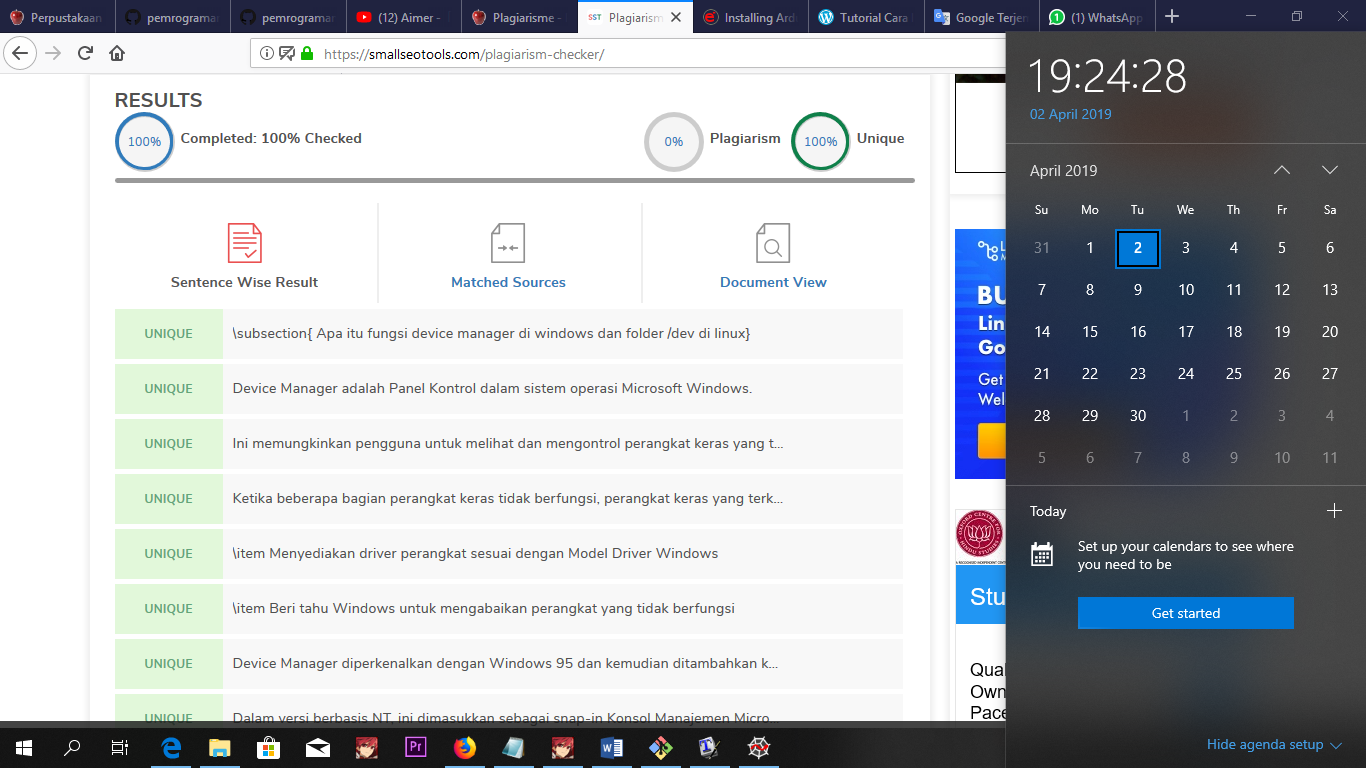
\includegraphics[scale=0.2]{figures/5/Teori/1174002/plagiat.png}
\caption{Plagiarisme}
\label{fig:plagiat}
\end{figure}

\section{Nico Ekklesia Sembiring}
\subsection{Apa itu fungsi device manager di windows dan folder /dev di linux}
berikut ini adalah fungsi device manager :
\begin{itemize}
	\item untuk menunjukkan status hardwarenya
	\item untuk menunjukkan informasi hardware secara detail
	\item Melakukan kelola driver pada hardware, seperti melakukan instalasi, uninstal, rollback, dan masalah lain yang berkaitan dengan driver.
	\item Melakukan identifikasi terhadap konflik yang terjadi pada hardware
\end{itemize}

Sedangkan folder /dev berisi file dari perangkat (Device), seperti device blok dan juga device karakter. Di dalam /dev minimal harus terdapat file biner MAKEDEV untuk dapat membuat device ini secara manual.
Di dalam sistem operasi Linux, setiap device yang tersambung akan dideteksi sebagai files, dan di dalam direktori /dev tersebut file-file khusus yang mempresentasikan perangkat tersimpan.

\subsection{Jelaskan langkah-langkah instalasi driver dari Arduino}
Berikut ini merupakan langkah-langkah untuk melakukan instalasi driver Arduino
\begin{itemize}
	\item Pertama-tama, pasang board arduino pada pc. Kemudian tunggu sampai windows mencoba menginstal sendiri. jika gagal, lanjutkan ke step selanjutnya
	\item buka Device Manager 
	\item Cari nama arduino atau "Unknown Device"
	\item klik kanan pada unknown device , dan pilih update software
	\item Cari folder instalan software arduino
	\item klik Next
	\item Jika telah berhasil, maka proses instal driver sudah selesai
\end{itemize}

\subsection{Jelaskan bagaimana cara membaca baudrate dan port dari komputer yang sudah terinstal driver}
Berikut ini merupakan cara membaca baudrate dan port dari komputer yang sudah terinstal driver :
\begin{itemize}
	\item Sambungkan port USB arduino dengan port USB pc
	\item Kemudian buka software arduino pada pc
	\item Setelah itu, pilih tipe arduino yang digunakan
	\item Kemudian memilih serial port yang aktif  
	\item Selanjutnya untuk memasukkan program pada arduino, klik tombol upload
	\item Setelah proses upload selesai, buka fitur serial monitor
	\item Lalu sesuaikan Baudrate pada serial monitor dengan Baudrate yang terdapat pada program
\end{itemize}

\subsection{Jelaskan sejarah library pyserial}
Pyserial berguna untuk merangkum akses untuk port serial. Pyserial menyediakan backends untuk Python yang berjalan di Windows, Linux, BSD (mungkin sistem yang mendukung POSIX), Jython dan IronPython (.NET dan Mono). Modul bernama "serial" secara otomatis memilih backend yang sesuai. Antarmuka berbasis kelas yang sama pada semua platform yang didukung.
Akses ke pengaturan port melalui properti Python.
Dukungan untuk berbagai ukuran byte, bit stop, paritas dan kontrol aliran dengan RTS / CTS dan / atau Xon / Xoff.
Bekerja dengan atau tanpa menerima batas waktu.
File seperti API dengan "read" dan "write" ("readline" dll. Juga didukung).
File-file dalam paket ini adalah 100 persen Python murni.
Port diatur untuk transmisi biner. Tidak ada stripping byte NULL, terjemahan CR-LF dll. (Yang berkali-kali diaktifkan untuk POSIX.) Ini membuat modul ini bermanfaat secara universal.
Kompatibel dengan pustaka io (Python 2.6+)

\subsection{Jelaskan fungsi-fungsi apa saja yang dipakai dari library pyserial}
Serial – fungsi ini untuk membuka port serial
Write(data) – untuk menulis data lewat port serial
Readline() – untuk membaca string dari port serial
Read(size) – untuk membaca jumlah byte dari port serial
Close() – ini untuk menutup port serial 

\subsection{Jelaskan kenapa butuh perulangan dalam tidak butuh perulangan dalam membaca serial}
Perualangan dalam bahasa pemrograman berfungsi menyuruh komputer melakukan sesuatu secara berulang-ulang. Terdapat dua jenis perualangan dalam bahasa pemrograman python, yaitu perulangan dengan for dan while.
Perulangan for disebut counted loop (perulangan yang terhitung), sementara perulangan while disebut uncounted loop (perulangan yang tak terhitung). Perbedaan yang terlihat adalah pada perulangan for digunakan untuk mengulangi kode yang sudah diketahui banyak perulangannya. Sedangkan perulangan while digunakan pada perulangan yang memiliki syarat dan tidak tentu berapa banyak perulangannya.
Perulangan diperlukan agar dapat membaca data secara berulang kali sehingga data yang muncul lebih dari satu.  Sedangkan apabila tidak memakai perulangan maka data akan terbaca satu kali saja.

\subsection{Jelaskan bagaimana cara membuat fungsi yang mengunakan pyserial}
Berikut merupakan contoh penggunaan fungsi yang menggunakan pyserial
\lstinputlisting[firstline=8, lastline=15]{src/5/teori/T1174096.py}


\subsection{Plagiarisme}
\begin{figure}[h]
\centering
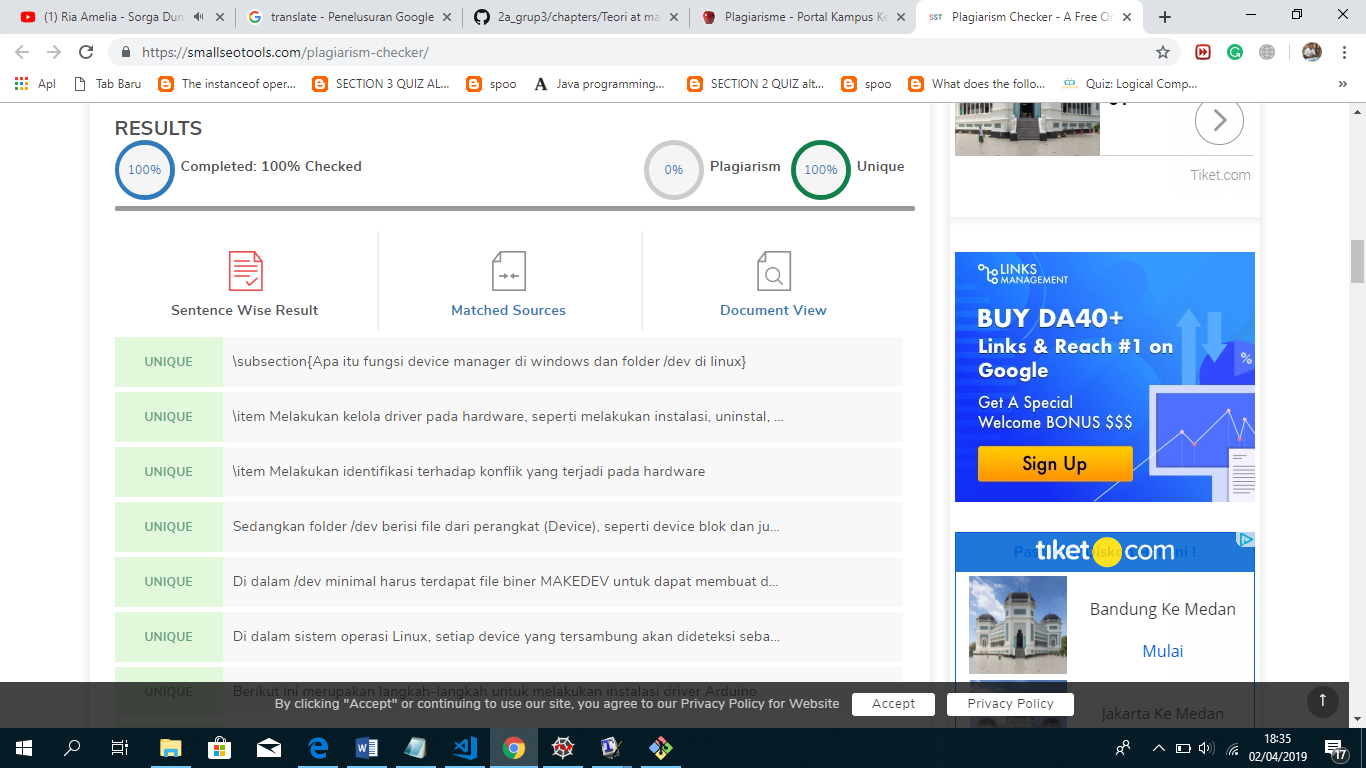
\includegraphics[scale=0.2]{figures/5/Teori/1174096/plagiat.png}
\caption{Plagiarisme}
\label{fig:plagiat}
\end{figure}

\section{Choirul Anam}
\subsection{Teori}
\subsubsection{Apa itu fungsi device manager di windows dan folder /dev di linux}
Fungsi device manager untuk membantu dan mengelola semua hardware yang terpasang dalam suatu windows.

\subsubsection{Jelaskan langkah-langkah instalasi driver dari arduino}
\begin{itemize}
    \item ubungkan sistem minimun Arduino Uno ke komputer dengan kabel USB type B (kabel Printer).
    \item Lalu pada bagian kanan didesktop PC anda, akan muncul popup “Installing device driver software”.
	\item Sistem operasi Windows tidak menyediakan driver untuk Arduino Uno, lalu proses instalasinya harus dilakukan secara manual.
	\item Buka Device Manager, caranya pada bagian Search Program and Files lalu ketikkan “device manager”.
	\item Cari Unknown device pada bagian Other device, terdapat tanda seru yang berwarna kuning, itu disebabkan karena penginstallan tidak berjalan dengan sempurna.
	\item Klik kanan pada “Unknown device”, pilih Update Driver Software.
    \item Pilih Browse my computer for driver software.
	\item Arahkan lokasi folder ke folder ..arduino-1.0.5 drivers. Pastikan check-box lalu centang include subfolders. Klik Next untuk melanjutkan instalasi driver.
	\item Kemudian lanjutkan dengan mengklik Install pada tampilan Windows Security.
	\item Jika instalasi driver berhasil maka akan muncul Windows has successfully updated your driver software.
	\item Perhatikan dan ingat nama COM Arduino Uno, karena nama COM ini yang akan digunakan untuk mengupload program nantinya.
\end{itemize}

\subsubsection{Jelaskan bagaimana cara membaca baudrate dan port dari komputer yang sudah terinstall driver}
Untuk baudrate dapat bisa dicek melalui arduino IDE, kemudian untuk mengecek port bisa dilakukan dengan device manager.

\subsubsection{Jelaskan sejarah library pyserial}
Modul ini merangkum akses untuk port serial. Ini menyediakan backends untuk Python yang berjalan di Windows, Linux, BSD (mungkin sistem yang mendukung POSIX), Jython dan IronPython (.NET dan Mono). Modul bernama "serial" secara otomatis memilih backend yang sesuai. Antarmuka berbasis kelas yang sama pada semua platform yang didukung.
Akses ke pengaturan port melalui properti Python. Dukungan untuk berbagai ukuran byte, bit stop, paritas dan kontrol aliran dengan RTS / CTS dan / atau Xon / Xoff. Bekerja dengan atau tanpa menerima batas waktu.
File seperti API dengan "read" dan "write" ("readline" dll. Juga didukung). File-file dalam paket ini adalah 100 persen Python murni. Port diatur untuk transmisi biner. Tidak ada stripping byte NULL, terjemahan CR-LF dll. (Yang berkali-kali diaktifkan untuk POSIX.) Ini membuat modul ini bermanfaat secara universal. Kompatibel dengan pustaka io (Python 2.6+)

\subsubsection{Jelaskan fungsi-fungsi apa saja yang dipakai dari library pyserial}
\begin{itemize}
    \item Serial – fungsi ini untuk membuka port serial
    \item Write(data) – untuk menulis data lewat port serial
    \item Readline() – untuk membaca string dari port serial
    \item Read(size) – untuk membaca jumlah byte dari port serial
    \item Close() – ini untuk menutup port serial 
\end{itemize}

\subsubsection{Jelaskan kenapa butuh perulangan dan tidak butuh perulangan dalam membaca serial}
Perualangan dalam bahasa pemrograman berfungsi untuk menyuruh komputer melakukan sesuatu secara berulang-ulang. Terdapat dua jenis perualangan dalam bahasa pemrograman python diantaranya adalah perulangan dengan for dan while.
Perulangan for atau counted loop (perulangan yang terhitung). Perulangan while atau uncounted loop (perulangan yang tak terhitung). Perbedaannya pada perulangan for biasanya digunakan untuk mengulangi kode yang sudah diketahui banyak perulangannya. Perualangan while untuk perulangan yang memiliki syarat dan tidak tentu berapa banyak perulangannya.
Perualangan digunakan untuk membaca data secara berulang-ulang  dan apabila tidak memakai perulangan, maka data akan terbaca satu per satu.

\subsubsection{Jelaskan bagaimana cara membuat fungsi yang mengunakan pyserial}
\lstinputlisting[firstline=8, lastline=15]{src/5/Teori/T1174004.py}

\subsection{Praktek}
\subsubsection{Kerjakan soal berikut ini, ....}
\subsubsection{Penanganan Error}

\section{Muhammad Dzihan Al-Banna}
\subsubsection{Soal 1}
Device Manager dalam system operasi Windows adalah perluasan dari Microsoft Management Console. Device Manager akan menampilkan seluruh hardware yang bisa diinisialisasi yang dikenal dengan system operasi Windows. Tampilannya terorganisir hingga dapatmemudahkan pengelolaan setiap hardware yang ada.
Fungsi-fungsi Device Manager antara lain sebagai berikut :
\begin{itemize}
\item Menunjukkan status suatu hardware
\item Menunjukkan informasi detail suatu hardware
\item Mengelola driver hardware
\item Disable \& Enable hardware
\item Meng-identifikasi konflik antar hardware, dll.
\end{itemize}
Directory pada /dev berisi file device, baik device blok maupun device karakter. di dalamnya sekurang-kurangnya  harus memiliki file biner MAKEDEV untuk membuat device ini secara manual.

\subsubsection{Soal 2}
\begin{itemize}
\item Hubungkan sistem minimun Arduino Uno ke komputer dengan kabel USB type B (kabel Printer).
\item Lalu pada bagian kanan didesktop PC anda, akan muncul popup “Installing device driver software” seperti pada gambar dibawah ini.
\item SIstem operasi Windows tidak menyediakan driver untuk Arduino Uno seperti yang terlihat pada gambar dibawah ini, lalu proses instalasinya harus dilakukan secara manual.
\item Buka Device Manager, caranya pada bagian Search Program and Files lalu ketikkan “device manager” (tanpa tanda petik), perhatikan gambar dibawah ini. Pada bagian Control Panel akan muncul Device Manager, klik untuk menjalankan.
\item Cari Unknown device pada bagian Other device, biasanya terdapat tanda seru berwarna kuning, itu disebabkan karena penginstallan tidak berjalan dengan sempurna.
\item Klik kanan pada “Unknown device” kemudian pilih Update Driver Software.
\item Pilih Browse my computer for driver software.
\item Arahkan lokasi folder ke folder arduino1.0.5 drivers. Pastikan checkbox lalu centang include subfolders. Klik Next untuk melanjutkan instalasi driver.
\item Kemudian lanjutkan dengan mengklik Install pada tampilan Windows Security.
\item Jika instalasi driver berhasil maka akan muncul Windows has successfully updated your driver software.
\item Perhatikan dan ingat nama COM Arduino Uno, karena nama COM ini yang akan digunakan untuk mengupload program nantinya.
\end{itemize}

\subsubsection{Soal 3}


Hubungkan Port USB pada Arduino dengan Port USB komputer.
Buka Software Arduino pada Komputer.
Tuliaskan program berikut ini pada Arduino Sketch.

\subsubsection{Soal 4}


Modul ini merangkum akses untuk port serial. Ini menyediakan backends untuk Python yang berjalan di Windows, Linux, BSD (mungkin sistem yang mendukung POSIX), Jython dan IronPython (.NET dan Mono). Modul bernama "serial" secara otomatis memilih backend yang sesuai. Antarmuka berbasis kelas yang sama pada semua platform yang didukung.
Akses ke pengaturan port melalui properti Python. 
Dukungan untuk berbagai ukuran byte, bit stop, paritas dan kontrol aliran dengan RTS / CTS dan / atau Xon / Xoff.
Bekerja dengan atau tanpa menerima batas waktu.
File seperti API dengan "read" dan "write" ("readline" dll. Juga didukung).
File-file dalam paket ini adalah 100 persen Phyton murni.
Port diatur untuk transmisi biner. Tidak ada stripping byte NULL, terjemahan CR-LF dll. (Yang berkali-kali diaktifkan untuk POSIX.) Ini membuat modul ini bermanfaat secara universal.
Kompatibel dengan pustaka io (Python 2.6+).

\subsubsection{Soal 5}


Fungsi-fungsi yang dipakai dari library Pyserial, diantara :
\begin{itemize}
\item Serial – fungsi ini untuk membuka port serial
\item Write(data) – untuk menulis data lewat port serial
\item Readline() – untuk membaca string dari port serial
\item Read(size) – untuk membaca jumlah byte dari port serial
\item Close() – ini untuk menutup port serial 
\end{itemize}

\subsubsection{Soal 6}


Perualangan dalam bahasa pemrograman berfungsi menyuruh komputer melakukan sesuatu secara berulang-ulang. Terdapat dua jenis perualangan dalam bahasa pemrograman python, yaitu perulangan dengan for dan while. Perulangan for disebut counted loop (perulangan yang terhitung), sementara perulangan while disebut uncounted loop (perulangan yang tak terhitung). Perbedaannya adalah perulangan for biasanya digunakan untuk mengulangi kode yang sudah diketahui banyak perulangannya. Sementara while untuk perulangan yang memiliki syarat dan tidak tentu berapa banyak perulangannya. Perulangan diperlukan agar dapat membaca data secara berulang kali sehingga data yang muncul lebih dari satu.  Sedangkan apabila tidak memakai perulangan maka data akan terbaca satu kali saja.

\subsubsection{Soal 7}


Berikut merupakan contoh penggunaan fungsi yang menggunakan pyserial
\lstinputlisting[firstline=8, lastline=15]{src/5/Teori/T1174095.py}

\subsubsection{Bukti bebas plagiarisme}
\begin{figure}[h]
\centering
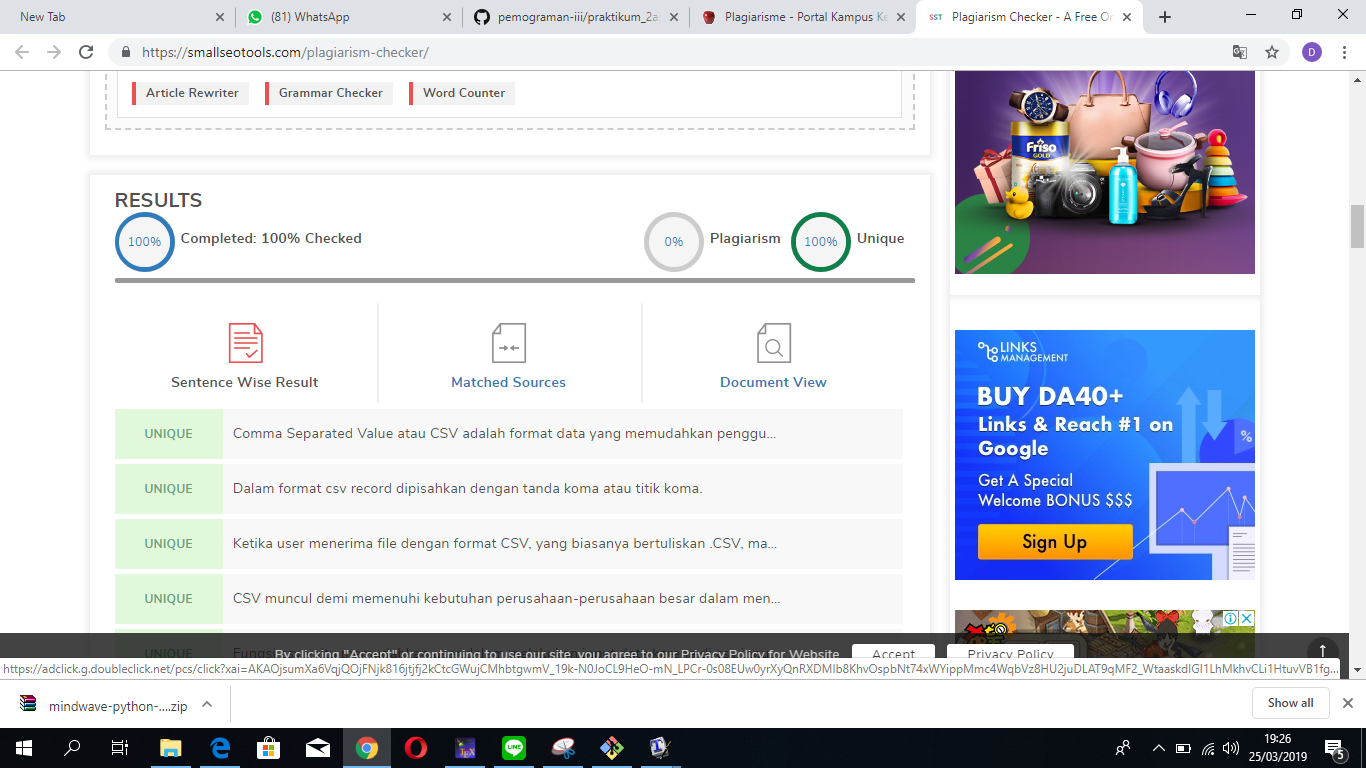
\includegraphics[width=10cm]{figures/5/Teori/1174095/1174095.png}
\caption{SS Bebas Plagiarisme}
\label{dzihan}
\end{figure}

\subsection{Praktek}
\subsubsection{Kerjakan soal berikut ini, ....}
\subsubsection{Penanganan Error}
Isi jawaban soal ke-1


%%%%%%%%%%%%%%%%%%%%%%%%%%%%%%%%%%%%%%%%%%%%%%%%%
\section{Oniwaldus Bere Mali}
\subsection{Teori}
\subsubsection{Apa itu fungsi device manager di windows dan folder /dev di linux}
Fungsi device manager dan folder /dev itu berfungsi untuk mengetahui device apa saja yang telah terinstal di leptop anda serta mengetahui port yang digunakan oleh device tersebut.

\subsubsection{Jelaskan langkah-langkah instalasi driver dari arduino}
\begin{enumerate}
\item Cara Auto
\begin{itemize}
\item Pertama Hubungkan sistem minimum Arduino Uno ke komputer dengan kabel USB type B(kabel Printer)
\begin{figure}[H] 
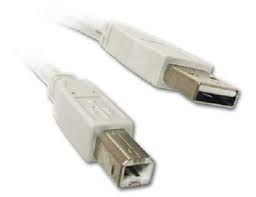
\includegraphics[width=5cm]{figures/5/Teori/1174005/1.jpg}
\centering
\caption{Membuat file csv}
\end{figure}

\item Lalu pada bagian kanan didesktop PC anda, akan muncul popup “Installing device driver software” seperti pada gambar dibawah ini.
\begin{figure}[H] 
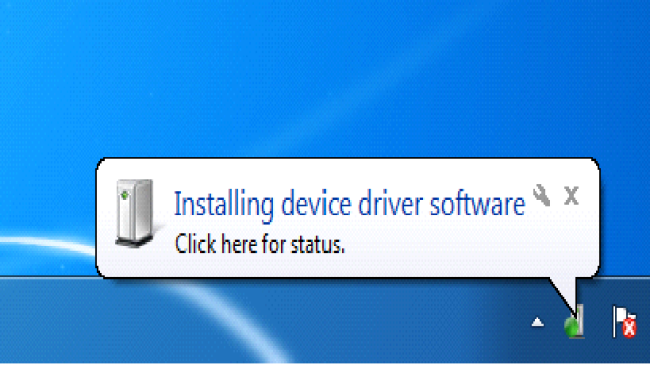
\includegraphics[width=5cm]{figures/5/Teori/1174005/2.png}
\centering
\caption{Membuat file csv}
\end{figure}

\item Tunggu hingga selesai.
\item Jika sudah selesai anda bisa mengecheck di device manager.
\begin{figure}[H] 
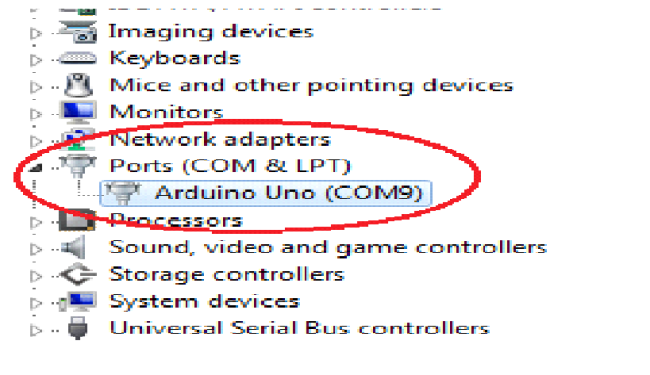
\includegraphics[width=5cm]{figures/5/Teori/1174005/11.png}
\centering
\caption{Membuat file csv}
\end{figure}
\end{itemize}

\item Cara Manual

\begin{itemize}
\item Penginstalan secara manual akan dilakukan jika penginstalan secara auto gagal dilakukan.
\item Buka Device Manager, caranya pada bagian Search Program and Files lalu ketikkan “device manager”, perhatikan gambar dibawah ini. Pada bagian Control Panel akan muncul Device Manager, klik untuk menjalankan.
\begin{figure}[H] 
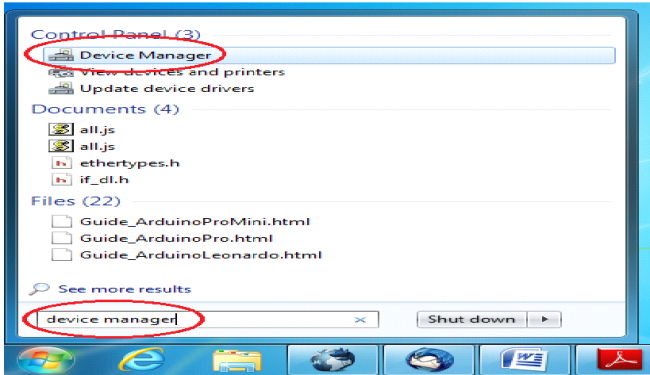
\includegraphics[width=5cm]{figures/5/Teori/1174005/4.png}
\centering
\caption{Membuat file csv}
\end{figure}

\item Cari Unknown device pada bagian Other device, biasanya terdapat tanda seru berwarna kuning, itu disebabkan karena penginstallan tidak berjalan dengan sempurna.
\begin{figure}[H] 
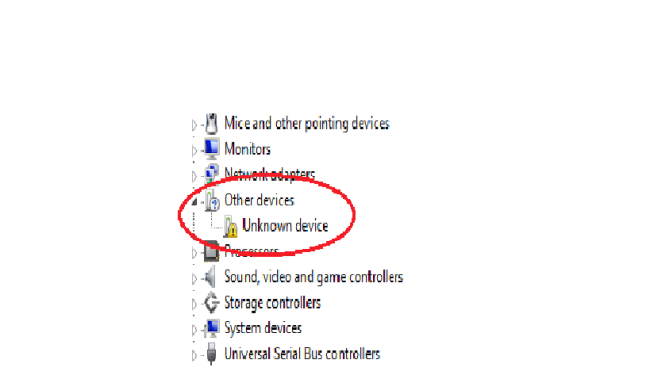
\includegraphics[width=5cm]{figures/5/Teori/1174005/5.png}
\centering
\caption{Membuat file csv}
\end{figure}

\item Klik kanan pada “Unknown device” kemudian pilih Update Driver Software.
\begin{figure}[H] 
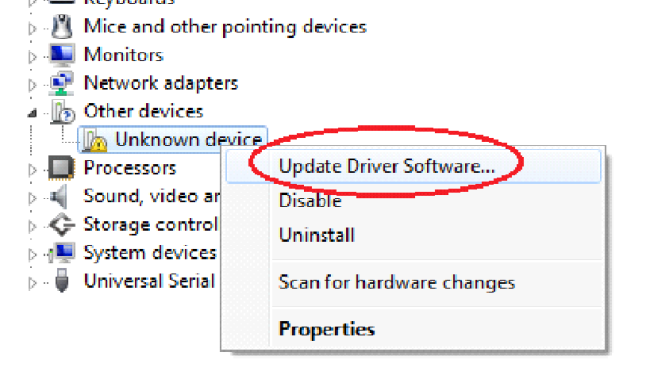
\includegraphics[width=5cm]{figures/5/Teori/1174005/6.png}
\centering
\caption{Membuat file csv}
\end{figure}

\item Pilih Browse my computer for driver software.
\begin{figure}[H] 
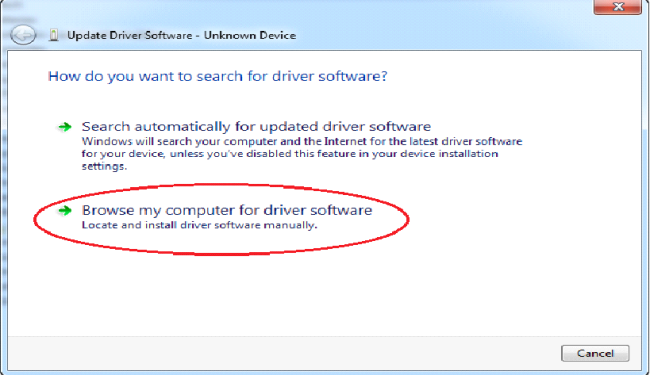
\includegraphics[width=5cm]{figures/5/Teori/1174005/7.png}
\centering
\caption{Membuat file csv}
\end{figure}

\item Arahkan lokasi folder ke folder ..arduino-1.0.5 drivers. Pastikan check-box lalu centang include subfolders. Klik Next untuk melanjutkan instalasi driver.
\begin{figure}[H] 
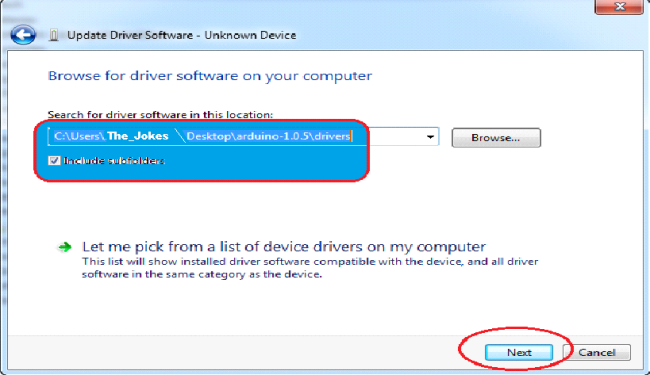
\includegraphics[width=5cm]{figures/5/Teori/1174005/8.png}
\centering
\caption{Membuat file csv}
\end{figure}

\item Kemudian lanjutkan dengan mengklik Install pada tampilan Windows Security.
\begin{figure}[H] 
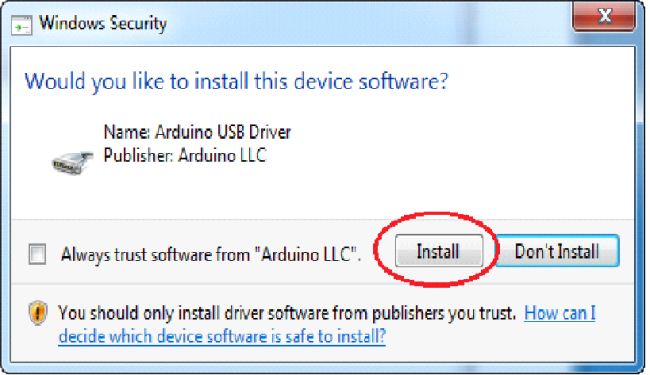
\includegraphics[width=5cm]{figures/5/Teori/1174005/9.png}
\centering
\caption{Membuat file csv}
\end{figure}

\item Jika instalasi driver berhasil maka akan muncul Windows has successfully updated your driver software.
\begin{figure}[H] 
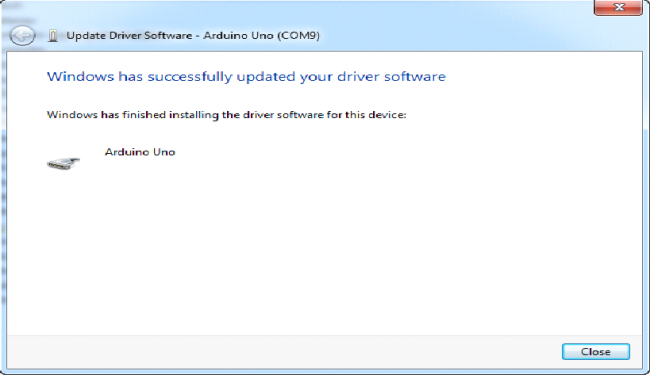
\includegraphics[width=5cm]{figures/5/Teori/1174005/10.png}
\centering
\caption{Membuat file csv}
\end{figure}

\item Perhatikan dan ingat nama COM Arduino Uno, karena nama COM ini yang akan digunakan untuk meng-upload program nantinya.
\begin{figure}[H] 
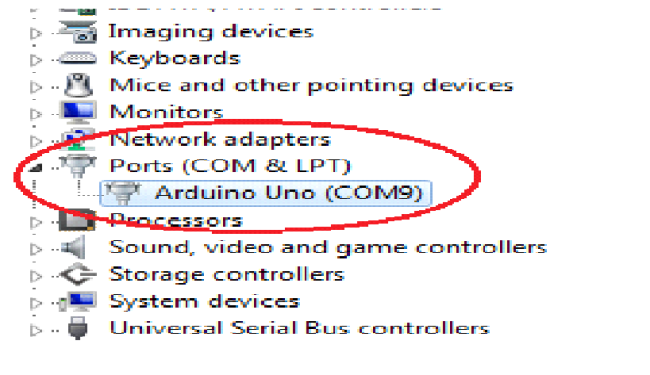
\includegraphics[width=5cm]{figures/5/Teori/1174005/11.png}
\centering
\caption{Membuat file csv}
\end{figure}
\end{itemize}
\end{enumerate}
\subsubsection{Jelaskan bagaimana cara membaca baudrate dan port dari komputer yang sudah terinstall driver}
Untuk baudrate itu bisa dicek melalui arduino IDE, kemudian untuk mengecheck port bisa dilakukan dengan device manager

\subsubsection{Jelaskan sejarah library pyserial}
Modul ini merangkum akses untuk port serial. Ini menyediakan backends untuk Python yang berjalan di Windows, Linux, BSD (mungkin sistem yang mendukung POSIX), Jython dan IronPython (.NET dan Mono). Modul bernama "serial" secara otomatis memilih backend yang sesuai. Antarmuka berbasis kelas yang sama pada semua platform yang didukung.
Akses ke pengaturan port melalui properti Python.
Dukungan untuk berbagai ukuran byte, bit stop, paritas dan kontrol aliran dengan RTS / CTS dan / atau Xon / Xoff.
Bekerja dengan atau tanpa menerima batas waktu.
File seperti API dengan "read" dan "write" ("readline" dll. Juga didukung).
File-file dalam paket ini adalah 100 persen Python murni.
Port diatur untuk transmisi biner. Tidak ada stripping byte NULL, terjemahan CR-LF dll. (Yang berkali-kali diaktifkan untuk POSIX.) Ini membuat modul ini bermanfaat secara universal.
Kompatibel dengan pustaka io (Python 2.6+)

\subsubsection{Jelaskan fungsi-fungsi apa saja yang dipakai dari library pyserial}


Serial – fungsi ini untuk membuka port serial
Write(data) – untuk menulis data lewat port serial
Readline() – untuk membaca string dari port serial
Read(size) – untuk membaca jumlah byte dari port serial
Close() – ini untuk menutup port serial 

\subsubsection{Jelaskan kenapa butuh perulangan dan tidak butuh perulangan dalam membaca serial}


Perualangan dalam bahasa pemrograman berfungsi menyuruh komputer melakukan sesuatu secara berulang-ulang. Terdapat dua jenis perualangan dalam bahasa pemrograman python, yaitu perulangan dengan for dan while.
Perulangan for disebut counted loop (perulangan yang terhitung), sementara perulangan while disebut uncounted loop (perulangan yang tak terhitung). Perbedaannya adalah perulangan for biasanya digunakan untuk mengulangi kode yang sudah diketahui banyak perulangannya. Sementara while untuk perulangan yang memiliki syarat dan tidak tentu berapa banyak perulangannya.
Perulangan diperlukan agar dapat membaca data secara berulang kali sehingga data yang muncul lebih dari satu. Sedangkan apabila tidak memakai perulangan maka data akan terbaca satu kali saja.

\subsubsection{Jelaskan bagaimana cara membuat fungsi yang mengunakan pyserial}


Berikut merupakan contoh penggunaan fungsi yang menggunakan pyserial
\lstinputlisting[firstline=8, lastline=15]{src/5/Teori/T1174005.py}

\subsubsection{Scan Plagiarisme}
\begin{figure}[H] 
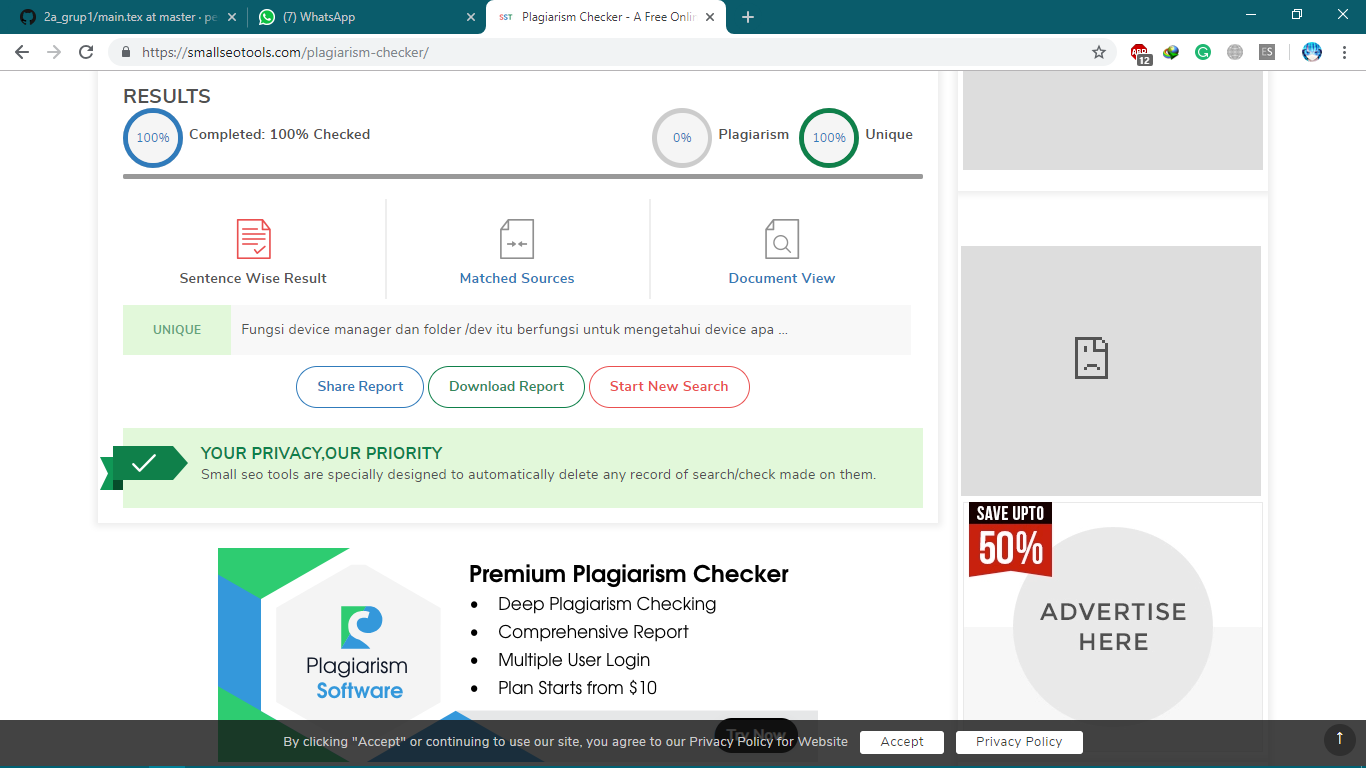
\includegraphics[width=5cm]{figures/5/Teori/1174005/nopla.png}
\centering
\caption{Membuat file csv}
\end{figure}

\subsection{Praktek}
\subsubsection{Kerjakan soal berikut ini, ....}
\subsubsection{Penanganan Error} 

%%%%%%%%%%%%%%%%%%%%%%%%%%%%%%%%%%%%%%%%%%%%%%%%%%%%%%%%%%%%%%
\section{Evietania Charis Sujadi}
{\Large \textbf{Pemahaman Teori}}
\subsection{Soal No. 1}
Apa itu fungsi device manager di windows dan folder /dev di linux?

\hfill \break
Fungsi device manager antara lain :
\begin{enumerate}
    \item Menunjukkan status suatu hardware.
    \item Menunjukkan informasi detil suatu hardware.
    \item Mengelola driver hardware
    \item Disable dan Enable hardware
    \item Mengidentifikasi konflik antar perangkat keras.
\end{enumerate}

\hfill \break
Folder /dev berisi file device, baik dari device blok maupun device karakter. Di dalamnya setidaknya ada file biner yang bernama MAKEDEV untuk membuat device secara manual.

\subsection{Soal No. 2}
Jelaskan langkah-langkah instalasi driver dari arduino!

\hfill \break
Berikut ini adalah langkah-langkah instalasi driver dari Arduino UNO di Windows:

\begin{enumerate}
    \item Hubungkan sistem minimun Arduino Uno ke komputer dengan kabel USB type B (kabel Printer).
    \item Lalu pada bagian kanan didesktop PC anda, akan muncul popup “Installing device driver software”.
    \item SIstem operasi Windows tidak menyediakan driver untuk Arduino Uno.
    \item Buka Device Manager, caranya pada bagian Search Program and Files lalu ketikkan “device manager” (tanpa tanda petik). Kemudian bagian Control Panel akan muncul halaman Device Manager, selanjutnya klik untuk menjalankan.
    \item Cari yang bernama Unknown device yang berada pada bagian Other device, biasanya ada tanda seru berwarna kuning, itu disebabkan karena penginstallan tidak berjalan dengan sempurna.
    \item Klik kanan pada “Unknown device” kemudian pilih Update Driver Software.
    \item Pilih Browse my computer for driver software.
    \item Arahkan lokasi folder ke folder ..arduino-1.0.5 drivers. Pastikan check-box lalu centang include subfolders. Klik Next untuk melanjutkan instalasi driver.
    \item Kemudian lanjutkan dengan mengklik Install pada tampilan Windows Security.
    \item Jika instalasi driver berhasil maka akan muncul Windows has successfully updated your driver software.
    \item Perhatikan dan ingat nama COM Arduino Uno, karena nama COM ini yang akan digunakan untuk meng-upload program nantinya.
\end{enumerate}

\subsection{Soal No. 3}
Jelaskan bagaimana cara membaca baudrate dan port dari komputer yang sudah terinstall driver!

\hfill \break
\textbf{Membaca Port dari Komputer}

\begin{enumerate}
    \item Hubungkan modul TX-RX serial dengan komputer melalui serial port menggunakan DB9 cable extension.
    \item Buka Hyper Terminal dengan menekan start kemudian All progams lalu Accessories kemudian Communications lalu Hyper Terminal.
    \item Ketik nama untuk Connection Description, misal coba, kemudian tekan OK.
    \item Pada Connect to, pilihlah COM port yang dipakai di Connect using, kemudian tekan OK.
    \item Masukkan nilai-nilai port settingnya, sesuai dengan DCE-nya. Kemudian tekan OK.
\end{enumerate}

\subsection{Soal No. 4}
Jelaskan sejarah library pyserial!

\hfill \break
PySerial adalah library/modul Python siap-pakai dan gratis yang dibuat untuk memudahkan kita dalam membuat program komunikasi data serial RS232 dalam bahasa Python.
Jika modul USB-2REL dapat kita kontrol dengan mudah menggunakan Python dan PyUSB, maka modul SER-2REL juga dapat kita kontrol dengan mudah menggunakan Python dengan bantuan modul PySerial.

\subsection{Soal No. 5}
Jelaskan fungsi-fungsi apa saja yang dipakai dari library pyserial!

\hfill \break
Fungsi-fungsi yang dipakai dari library PySerial, yaitu:
\begin{enumerate}
    \item Serial - fungsi ini untuk membuka port serial.
    \item write(data) - fungsi ini menulis data lewat port serial.
    \item readline() - fungsi ini membaca sebuah string dari port serial.
    \item read(size) - fungsi ini untuk membaca jumlah byte dari port serial.
    \item close() - fungsi ini untuk menutup port serial.
\end{enumerate}

\subsection{Soal No. 6}
Jelaskan kenapa butuh perulangan dan tidak butuh perulangan dalam membaca serial!

\hfill \break
Pada saat membaca serial di Arduino diperlukan perulangan agar bisa membaca data secara berulang kali sehingga data yang muncul banyak. Sedangkan apabila tidak membutuhkan perulangan maka Arduino hanya akan membaca data sekali saja.

\subsection{Soal No. 7}
Jelaskan bagaimana cara membuat fungsi yang mengunakan pyserial!

\hfill \break
Fungsi yang berada pada Python, dibuat dengan nama kata kunci def kemudian diikuti dengan nama fungsinya pada pyhton.
Seperti halnya dengan blok kode yang lain, kita juga harus memberikan identasi untuk menuliskan isi fungsi.

\subsubsection{Bukti bebas plagiarisme}
\begin{figure}[h]
\centering
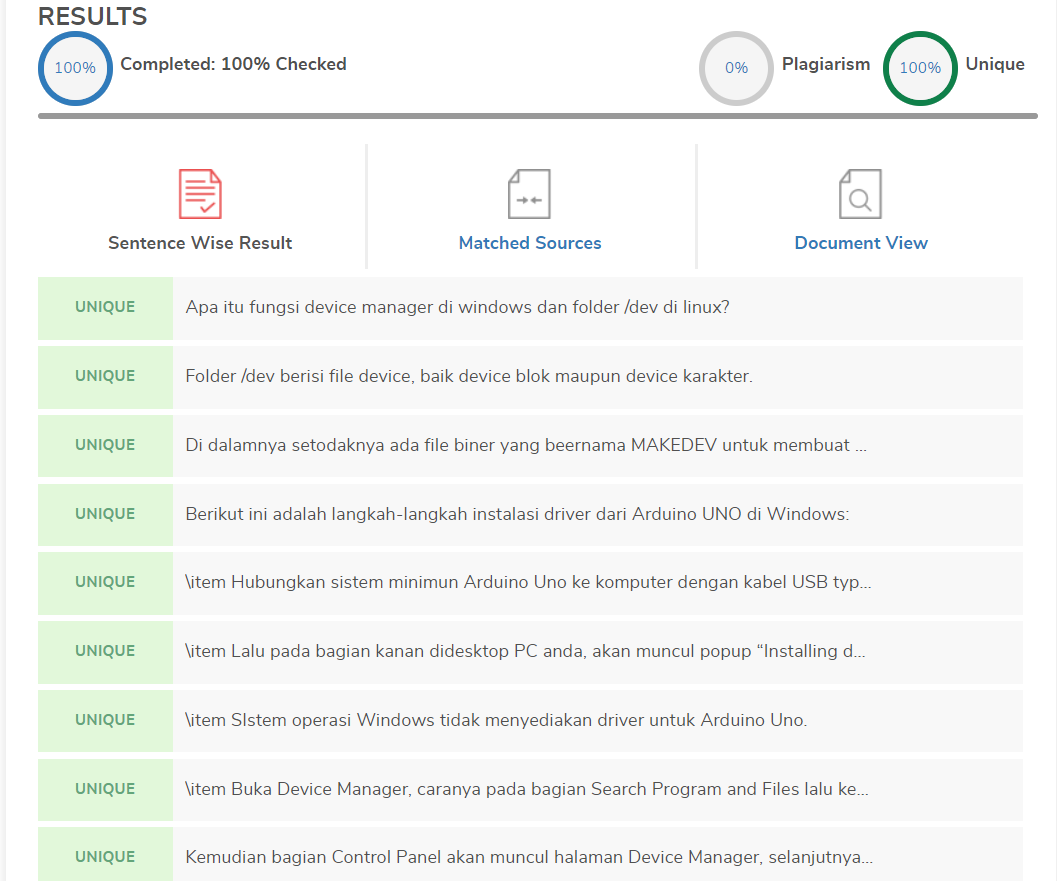
\includegraphics[width=10cm]{figures/5/Teori/1174051/Plagiat.png}
\caption{Bebas Plagiarisme}
\label{Evietania}
\end{figure}

%%%%%%%%%%%%%%%%%%%%%%%%%%%%%%%%%%%%%%%%%%%%%%%%%%%%%%%%%%%%%%%%%%%

\section{Dezha Aidil Martha}
\subsection{Bagian 1 - Teori}
\subsubsection{Apa itu fungsi device manager di windows dan folder /dev di linux}
Fungsi device manager dan folder /dev itu berfungsi untuk mengetahui device apa saja yang telah terinstal di leptop anda serta mengetahui port yang digunakan oleh device tersebut.

\subsubsection{Jelaskan langkah-langkah instalasi driver dari arduino}
\begin{enumerate}
\item Cara Auto
\begin{itemize}
\item Pertama Hubungkan sistem minimum Arduino Uno ke komputer dengan kabel USB type B(kabel Printer)
\begin{figure}[H] 
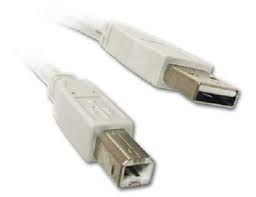
\includegraphics[width=5cm]{figures/5/Teori/1174025/no1.jpg}
\centering
\caption{Koneksikan Arduino Uno menggunakan kabel}
\end{figure}

\item Lalu pada bagian kanan didesktop PC anda, akan muncul popup “Installing device driver software” seperti pada gambar dibawah ini.
\begin{figure}[H] 
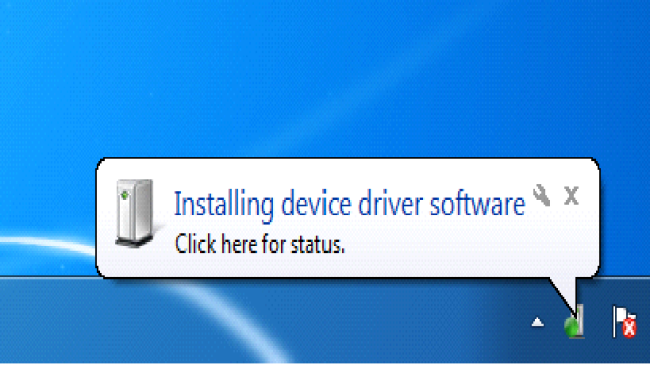
\includegraphics[width=5cm]{figures/5/Teori/1174025/no2.png}
\centering
\end{figure}

\item Tunggu hingga selesai.
\item Jika sudah selesai anda bisa mengecheck di device manager.
\begin{figure}[H] 
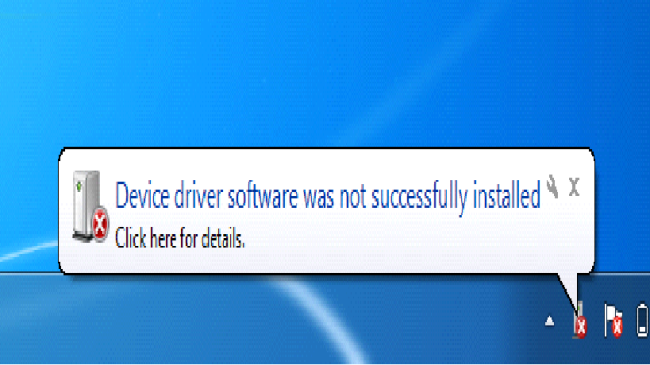
\includegraphics[width=5cm]{figures/5/Teori/1174025/no3.png}
\centering
\caption{Cek driver sudah terinstall atau belum}
\end{figure}
\end{itemize}

\item Cara Manual
\begin{itemize}
\item Penginstalan secara manual akan dilakukan jika penginstalan secara auto gagal dilakukan.
\item Buka Device Manager, caranya pada bagian Search Program and Files lalu ketikkan “device manager”, perhatikan gambar dibawah ini. Di bagian Control Panel akan muncul Device Manager, klik untuk menjalankan.
\begin{figure}[H] 
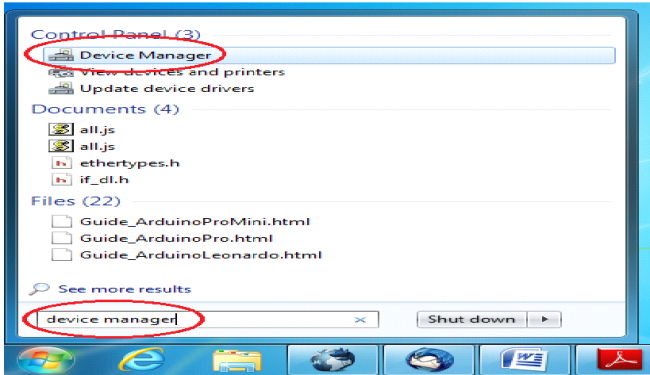
\includegraphics[width=5cm]{figures/5/Teori/1174025/no4.png}
\centering
\caption{Instalasi driver secara manual}
\end{figure}

\item Cari Unknown device pada bagian Other device, pada umumnya terdapat tanda seru berwarna kuning, itu disebabkan karena penginstallan tidak berjalan dengan lancar.
\begin{figure}[H] 
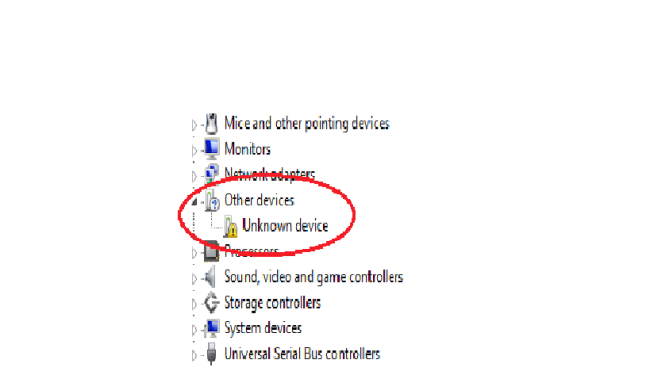
\includegraphics[width=5cm]{figures/5/Teori/1174025/no5.png}
\centering
\end{figure}

\item Klik kanan pada “Unknown device” kemudian pilih Update Driver Software.
\begin{figure}[H] 
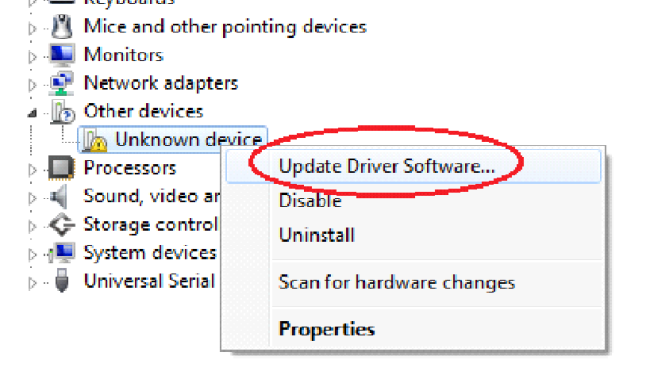
\includegraphics[width=5cm]{figures/5/Teori/1174025/no6.png}
\centering
\end{figure}

\item Lalu Pilih Browse my computer for driver software.
\begin{figure}[H] 
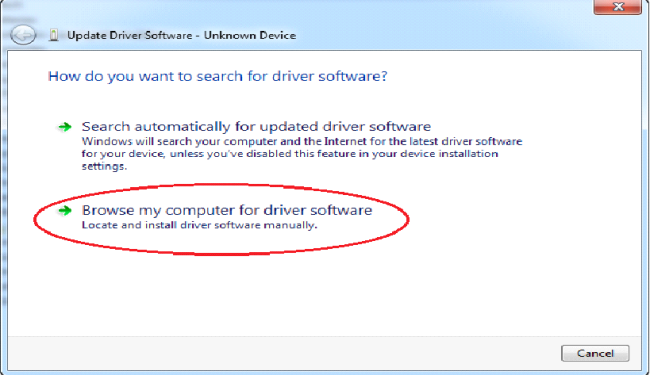
\includegraphics[width=5cm]{figures/5/Teori/1174025/no7.png}
\centering
\end{figure}

\item Arahkan lokasi folder ke folder ..arduino-1.0.5 drivers. Pastikan check-box lalu centang include subfolders. Klik Next untuk melanjutkan instalasi driver.
\begin{figure}[H] 
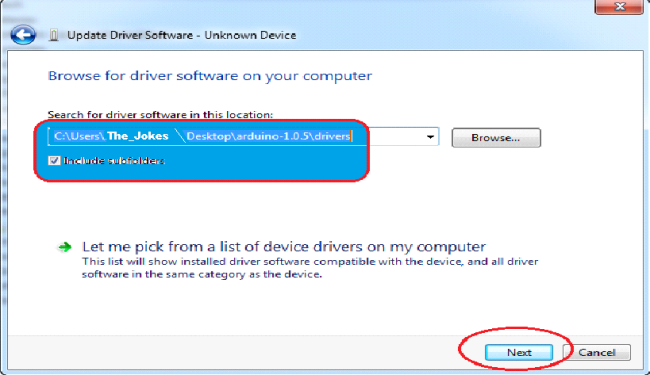
\includegraphics[width=5cm]{figures/5/Teori/1174025/no8.png}
\centering
\end{figure}

\item Kemudian lanjutkan dengan mengklik Install pada tampilan Windows Security.
\begin{figure}[H] 
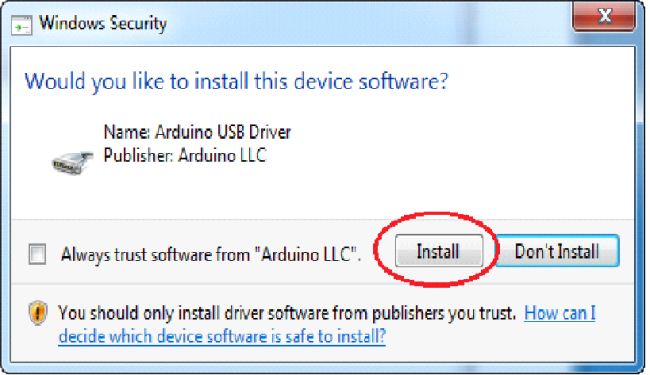
\includegraphics[width=5cm]{figures/5/Teori/1174025/no9.png}
\centering
\end{figure}

\item Jika instalasi driver berhasil maka akan muncul Windows has successfully updated your driver software.
\begin{figure}[H] 
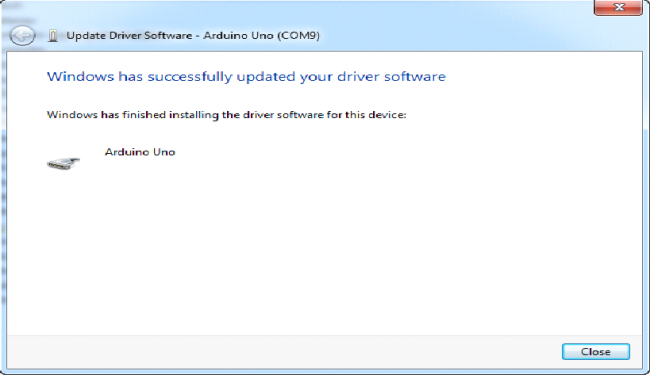
\includegraphics[width=5cm]{figures/5/Teori/1174025/no10.png}
\centering
\end{figure}

\item Perhatikan dan ingat nama COM Arduino Uno, karena nama COM ini yang akan digunakan untuk meng-upload program nantinya.
\begin{figure}[H] 
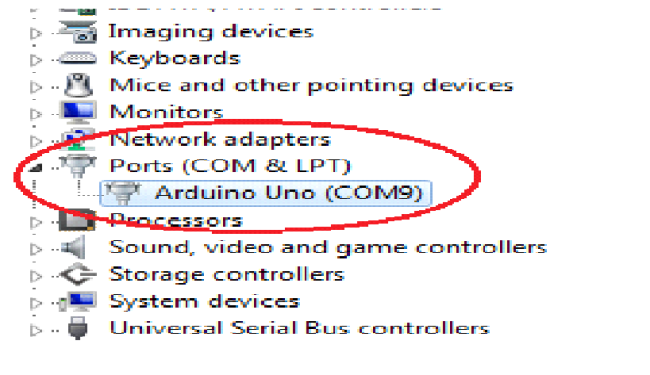
\includegraphics[width=5cm]{figures/5/Teori/1174025/no11.png}
\centering
\end{figure}
\end{itemize}
\end{enumerate}
\subsubsection{Jelaskan bagaimana cara membaca baudrate dan port dari komputer yang sudah terinstall driver}
Untuk baudrate itu bisa dicek melalui arduino IDE, kemudian untuk mengecheck port bisa dilakukan dengan device manager

\subsubsection{Jelaskan sejarah library pyserial}
Modul ini merangkum akses untuk port serial. Ini menyediakan backends untuk Python yang berjalan di Windows, Linux, BSD (mungkin sistem yang mendukung POSIX), Jython dan IronPython (.NET dan Mono). Modul bernama "serial" secara otomatis memilih backend yang sesuai. Antarmuka berbasis kelas yang sama pada semua platform yang didukung.
Akses ke pengaturan port melalui properti Python.
Dukungan untuk berbagai ukuran byte, bit stop, paritas dan kontrol aliran dengan RTS / CTS dan / atau Xon / Xoff.
Bekerja dengan atau tanpa menerima batas waktu.
File seperti API dengan "read" dan "write" ("readline" dll. Juga didukung).
File-file dalam paket ini adalah 100 persen Python murni.
Port diatur untuk transmisi biner. Tidak ada stripping byte NULL, terjemahan CR-LF dll. (Yang berkali-kali diaktifkan untuk POSIX.) Ini membuat modul ini bermanfaat secara universal.
Kompatibel dengan pustaka io (Python 2.6+)

\subsubsection{Jelaskan fungsi-fungsi apa saja yang dipakai dari library pyserial}


Serial – fungsi ini untuk membuka port serial
Write(data) – untuk menulis data lewat port serial
Readline() – untuk membaca string dari port serial
Read(size) – untuk membaca jumlah byte dari port serial
Close() – ini untuk menutup port serial 

\subsubsection{Jelaskan kenapa butuh perulangan dan tidak butuh perulangan dalam membaca serial}


Perualangan dalam bahasa pemrograman berfungsi menyuruh komputer melakukan sesuatu secara berulang-ulang. Terdapat dua jenis perualangan dalam bahasa pemrograman python, yaitu perulangan dengan for dan while.
Perulangan for disebut counted loop (perulangan yang terhitung), sementara perulangan while disebut uncounted loop (perulangan yang tak terhitung). Perbedaannya ialah, perulangan (for) biasanya dipakai untuk mengulangi kode yang sudah diketahui banyak perulangannya. Sementara itu, perulangan (while) dipakai untuk perulangan yang memiliki syarat dan tidak tentu berapa banyak perulangannya.
Perulangan diperlukan agar dapat membaca data secara berulang kali sehingga data yang muncul lebih dari satu. Sedangkan apabila tidak memakai perulangan maka data akan terbaca satu kali saja.

\subsubsection{Jelaskan bagaimana cara membuat fungsi yang mengunakan pyserial}


Berikut merupakan contoh penggunaan fungsi yang menggunakan pyserial
\lstinputlisting[firstline=8, lastline=15]{src/5/Teori/T1174025.py}

\subsubsection{Scan Plagiarisme}
\begin{figure}[H] 
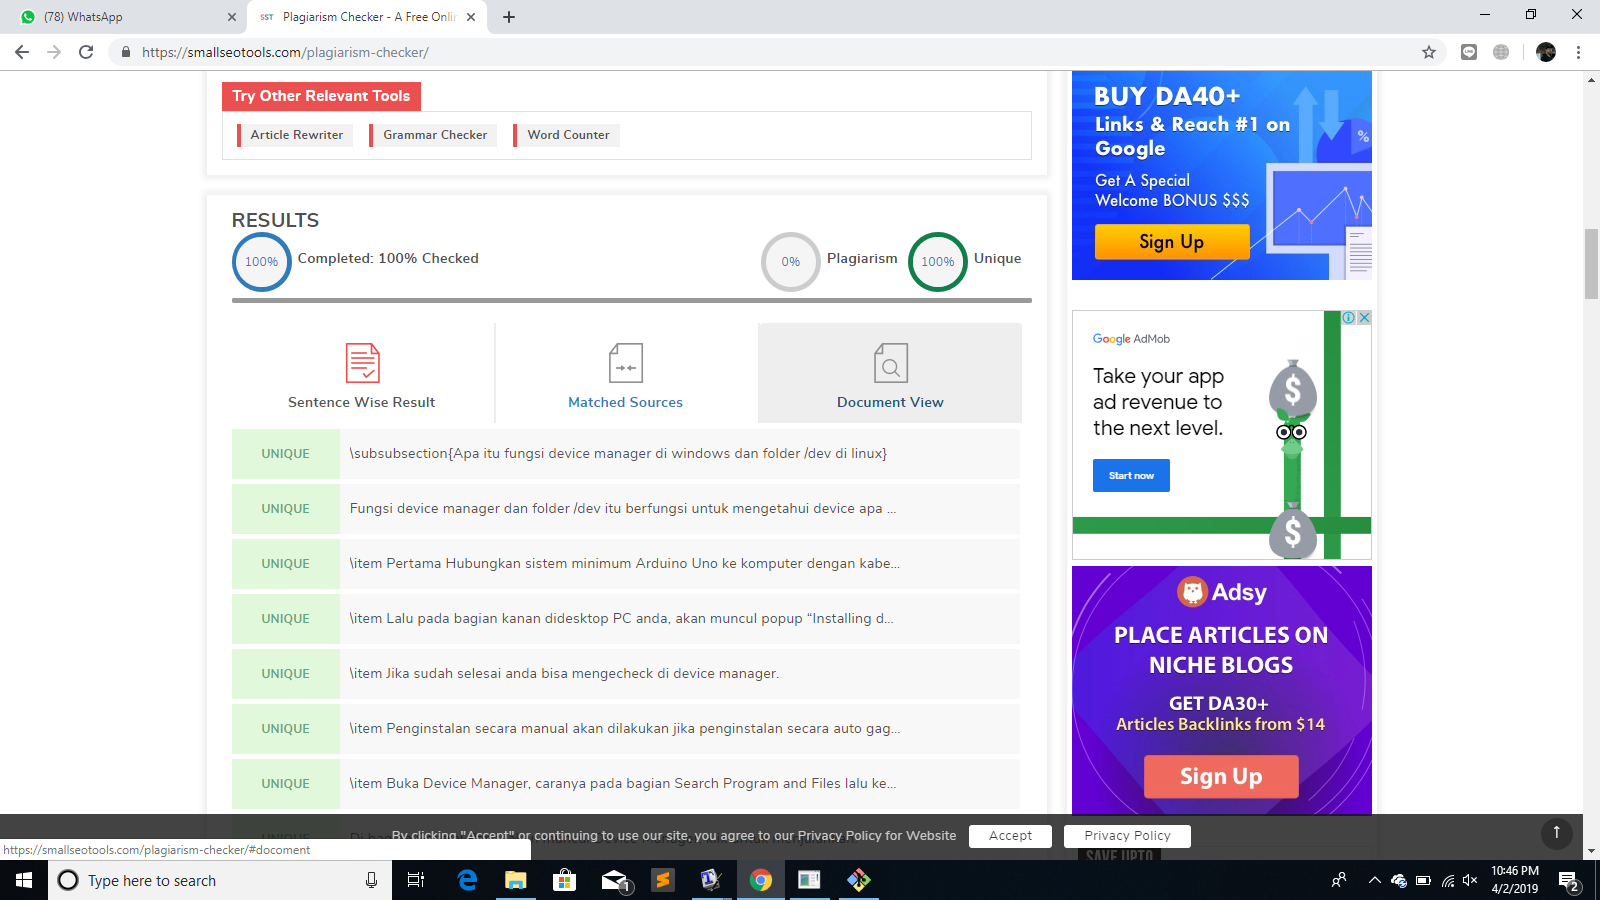
\includegraphics[width=5cm]{figures/5/Teori/1174025/noplg.png}
\centering
\end{figure}
%PRAKTEK
\chapter{Praktek Komunikasi Perangkat Keras}

\section{Nico Ekklesia Sembiring}
\subsection{Buatlah fungsi untuk mendapatkan data langsung dari arduino}
\lstinputlisting[caption = Mendapatkan data dari Arduino., firstline=8, lastline=14]{src/5/Praktek/1174096/1174096_realtime.py}

\subsection{Buatlah fungsi untuk mendapatkan data langsung dari arduino dengan looping}
\lstinputlisting[caption = Mendapatkan data langsung dari Arduino dengan looping., firstline=8, lastline=15]{src/5/Praktek/1174096/1174096_save.py}

\subsection{Buatlah fungsi untuk mendapatkan data dari arduino dan langsung ditulis kedalam file csv}
\lstinputlisting[caption = Mendapatkan data dari Arduino dan langsung ditulis kedalam file CSV., firstline=16, lastline=30]{src/5/Praktek/1174096/1174096_realtime.py}

\begin{figure}[H]
	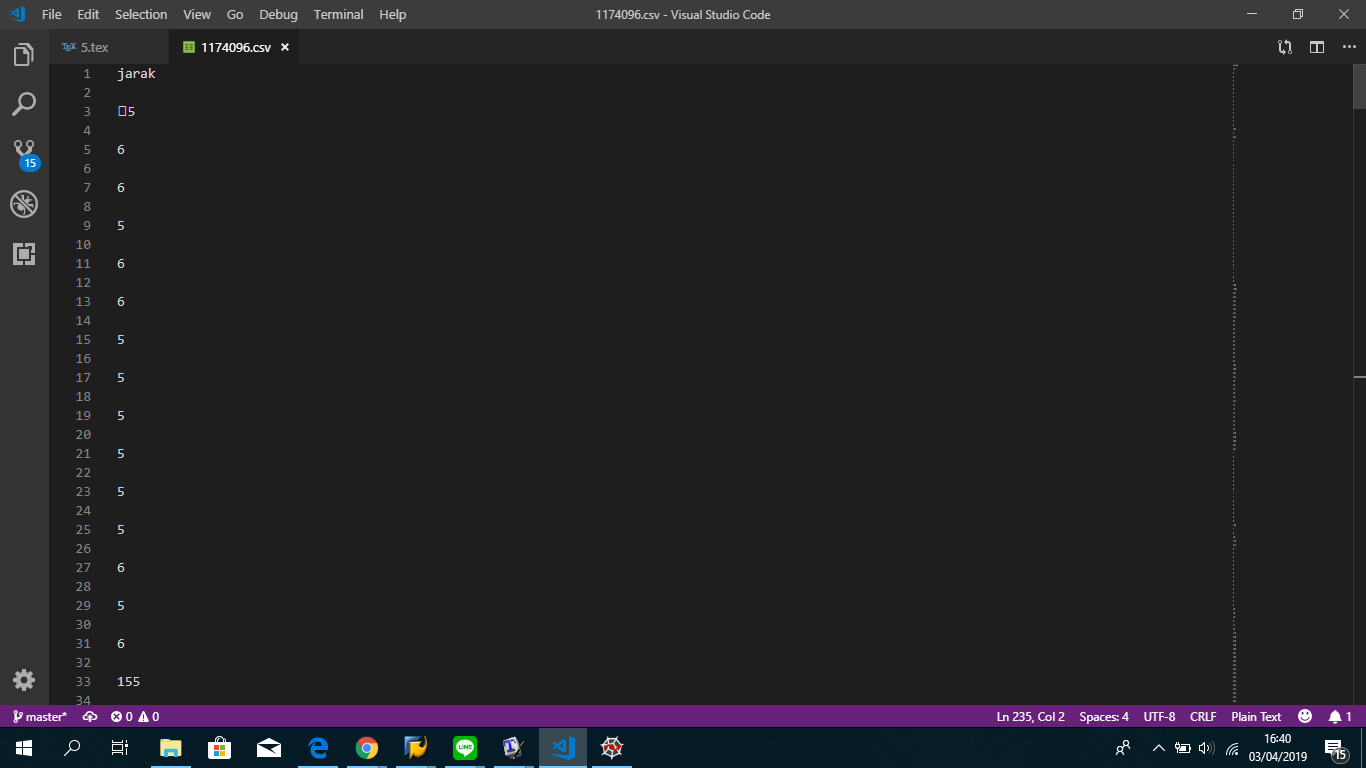
\includegraphics[width=9cm]{figures/5/Praktek/1174096/hasilcsv.png}
	\caption{Hasil dari pembacaan data dari arduino dalam bentuk file CSV.}
	\centering
\end{figure}

\subsection{Buatlah fungsi untuk membaca file csv hasil arduino dan mengembalikan ke fungsi}
\lstinputlisting[caption = Membaca file CSV hasil Arduino dan mengembalikan fungsi., firstline=8, lastline=16]{src/5/Praktek/1174096/1174096_csv.py}

\subsection{Pengecekan Plagiarisme Praktek}
\begin{figure}[H]
	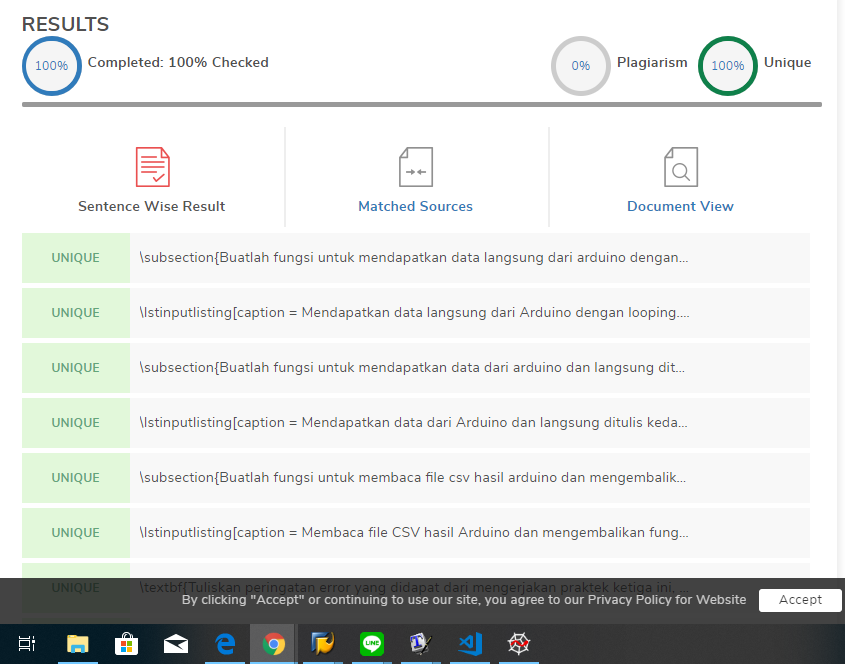
\includegraphics[width=9cm]{figures/5/Praktek/1174096/Plagiarismepraktek.png}
	\centering
\end{figure}

\subsection{Ketrampilan Penanganan Error}
\textbf{Tuliskan peringatan error yang didapat dari mengerjakan praktek ketiga ini, dan jelaskan cara penanganan error tersebut. dan Buatlah satu fungsi yang menggunakan gunakan try except untuk menanggulangi error tersebut}

Peringatan error yang saya temui pada praktek Chapter 5 ini, adalah:
\begin{itemize}
	\item Name Error
	NameError adalah exception yang terjadi ketika kode melakukan eksekusi terhadap local name atau global name yang tidak terdefinisi oleh perangkat. Solusi yang dapat dilakukan adalah dengan memastikan variabel atau fungsi yang dipanggil ada atau tidak salah ketik.
	
	\item Syntax Errors
	Syntax Errors adalah suatu keadaan saat  terjadi kesalahan penulisan pada kode python. Cara memperbaikinya adalah dengan memperbaiki penulisan kode yang salah.
	
	\item Type Error
	TypeError adalah exception yang terjadi pada saat dilakukannya eksekusi terhadap suatu operasi atau fungsi dengan type object yang tidak sesuai. Cara yang dilakukan untuk mengatasinya error ini adalah mengkoversi varibelnya sesuai dengan tipe data yang akan digunakan.
\end{itemize}

\textbf{Penanggulangan Error menggunakan Try Except}
\lstinputlisting[caption = Penanggulangan error menggunakan Try Except., firstline=8, lastline=23]{src/5/Praktek/1174096/1174096.py}

\subsection{Pengecekan Plagiarisme Penanganan Error}
\begin{figure}[H]
	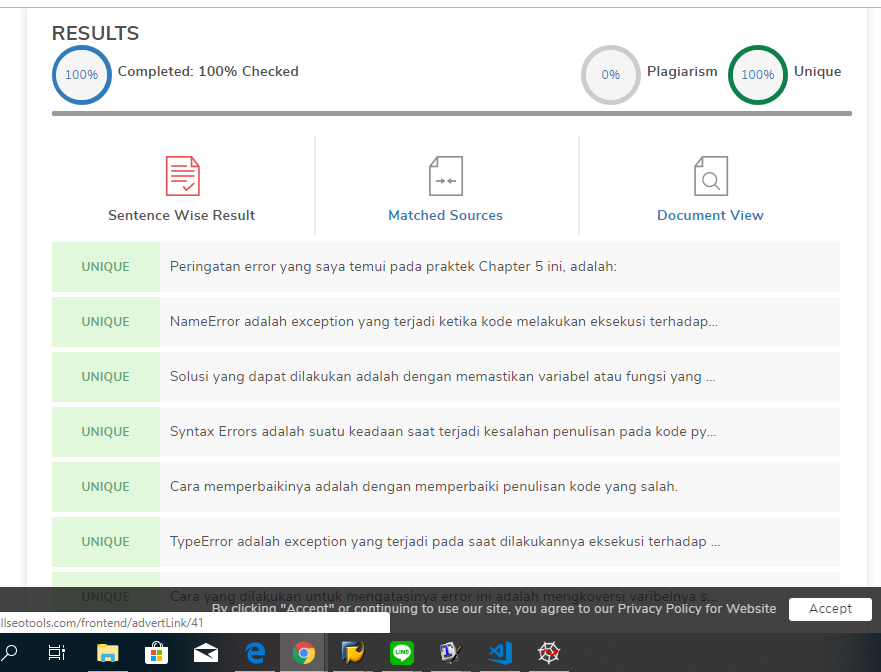
\includegraphics[width=9cm]{figures/5/Praktek/1174096/Plagiarismeerror.png}
	\centering
\end{figure}

\section{Habib Abdul Rasyid}
{\Large \textbf{Ketrampilan Pemrograman}}
\subsection{Soal No. 1}
Buatlah  fungsi  (file  terpisah/library  dengan  nama  NPMrealtime.py)  untuk mendapatkan data langsung dari arduino!
\lstinputlisting[caption = Fungsi untuk mendapatkan data dari Arduino., firstline=1, lastline=14]{src/5/Praktek/1174002/1174002realtime.py}


\subsection{Soal No. 2}
Buatlah fungsi (file terpisah/library dengan nama NPMsave.py) untuk mendapatkan data langsung dari arduino dengan looping!
\lstinputlisting[caption = Fungsi untuk mendapatkan data langsung dari Arduino dengan looping., firstline=1, lastline=8]{src/5/Praktek/1174002/1174002save.py}

\subsection{Soal No. 3}
Buatlah  fungsi  (file  terpisah/library  dengan  nama  NPMrealtime.py) untuk mendapatkan data dari arduino dan langsung ditulis kedalam file csv!
\lstinputlisting[caption = Fungsi untuk mendapatkan data dari Arduino dan langsung ditulis kedalam file CSV., firstline=16, lastline=30]{src/5/Praktek/1174002/1174002realtime.py}

\begin{figure}[H]
	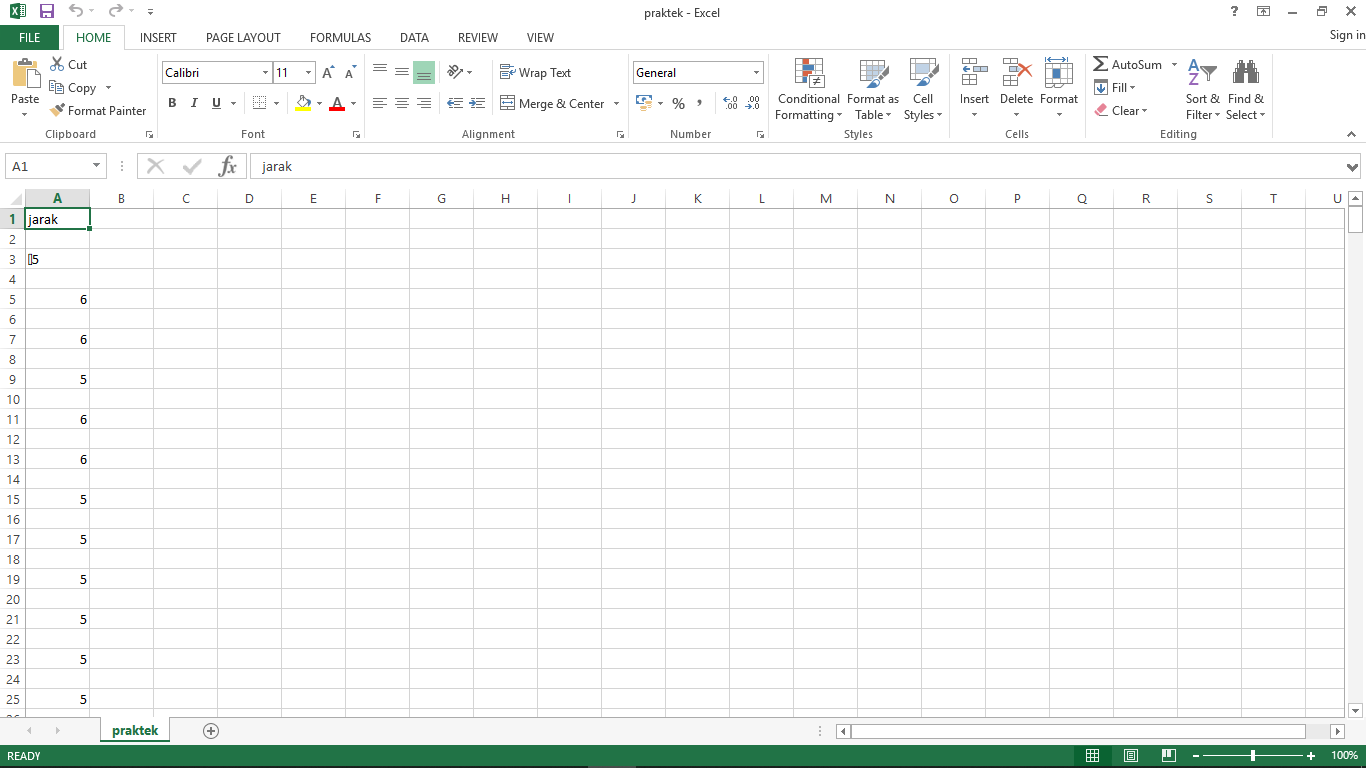
\includegraphics[scale=0.2]{figures/5/Praktek/1174002/csv.png}
	\centering
	\caption{Hasil dari pembacaan fungsi untuk mendapatkan data dari Arduino dan langsung ditulis kedalam file CSV.}
\end{figure}

\subsection{Soal No. 4}
Buatlah fungsi (file terpisah/library dengan nama NPMcsv.py) untuk membaca file csv hasil arduino dan mengembalikan ke fungsi!
\lstinputlisting[caption = Fungsi untuk membaca file CSV hasil Arduino dan mengembalikan fungsi., firstline=1, lastline=9]{src/5/Praktek/1174002/1174002csv.py}

\subsection{Cek Plagiat Praktek}
\begin{figure}[H]
	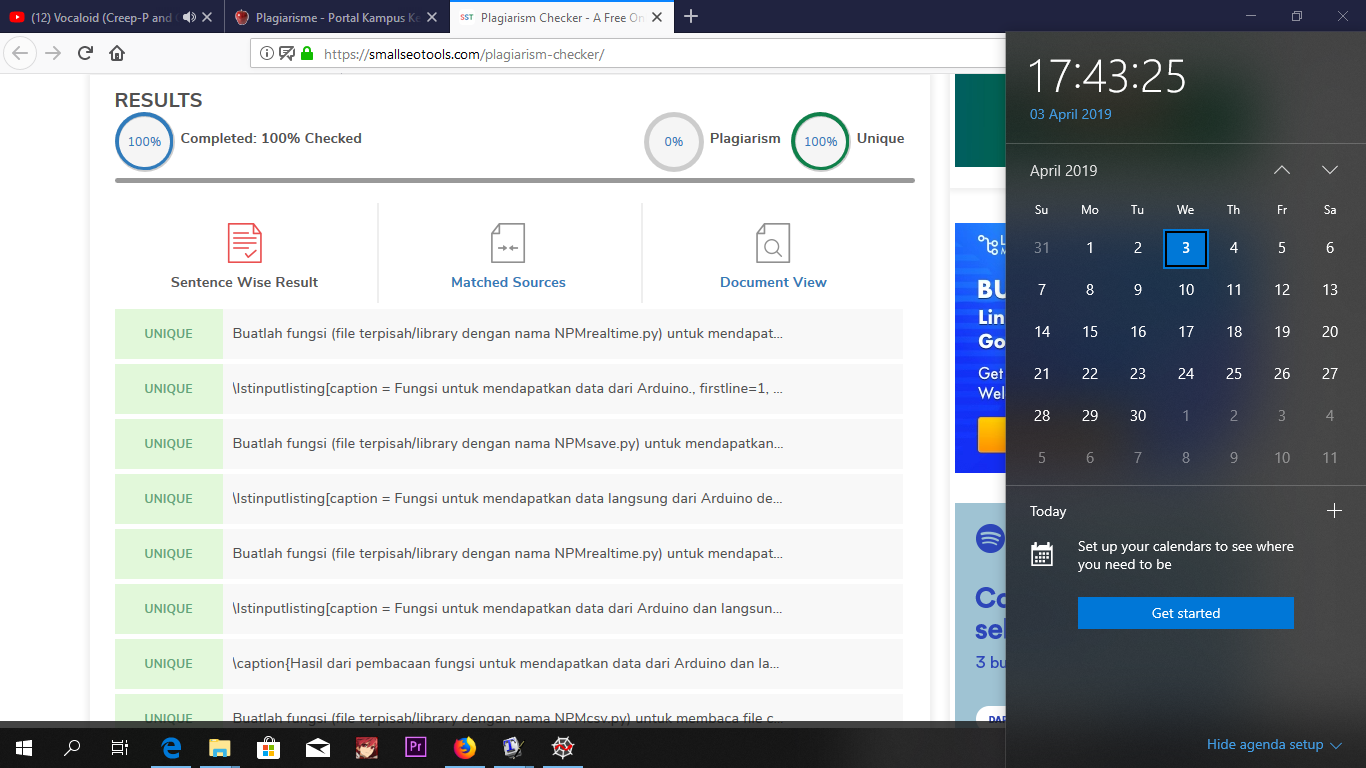
\includegraphics[scale=0.2]{figures/5/Praktek/1174002/plagiat.png}
	\caption{Plagiarisme Habib}
	\centering
\end{figure}

\hfill \break
{\Large \textbf{Ketrampilan Penanganan Error}}

\subsection{Soal No. 1}
Tuliskan  peringatan  error  yang  didapat  dari  mengerjakan  praktek  kelima  ini, dan  jelaskan  cara  penanganan  error  tersebut.   dan  Buatlah  satu  fungsi  yang menggunakan try except untuk menanggulangi error tersebut.

\hfill \break
Peringatan error di praktek kelima ini, yaitu:
\begin{itemize}
	\item Syntax Errors
	Syntax Errors adalah suatu keadaan saat kode python mengalami kesalahan penulisan. Solusinya adalah memperbaiki penulisan kode yang salah.
		
	\item Type Error
	TypeError adalah exception yang akan terjadi apabila pada saat dilakukannya eksekusi terhadap suatu operasi atau fungsi dengan type object yang tidak sesuai. Solusi dari error ini adalah mengkoversi varibelnya sesuai dengan tipe data yang akan digunakan.
\end{itemize}

\hfill \break
Fungsi yang menggunakan try except untuk menanggulangi error.

\lstinputlisting[caption = Fungsi untuk menanggulangi error menggunakan Try Except., firstline=1, lastline=16]{src/5/Praktek/1174002/1174002.py}

\section{Choirul Anam}
{\Large \textbf{Ketrampilan Pemrograman}}
\subsection{Soal No. 1}
Buatlah  fungsi  (file  terpisah/library  dengan  nama  NPMrealtime.py)  untuk mendapatkan data langsung dari arduino!
\lstinputlisting[caption = Fungsi untuk mendapatkan data dari Arduino., firstline=1, lastline=14]{src/5/Praktek/1174004/1174004realtime.py}


\subsection{Soal No. 2}
Buatlah fungsi (file terpisah/library dengan nama NPMsave.py) untuk mendapatkan data langsung dari arduino dengan looping!
\lstinputlisting[caption = Fungsi untuk mendapatkan data langsung dari Arduino dengan looping., firstline=1, lastline=8]{src/5/Praktek/1174004/1174004save.py}

\subsection{Soal No. 3}
Buatlah  fungsi  (file  terpisah/library  dengan  nama  NPMrealtime.py) untuk mendapatkan data dari arduino dan langsung ditulis kedalam file csv!
\lstinputlisting[caption = Fungsi untuk mendapatkan data dari Arduino dan langsung ditulis kedalam file CSV., firstline=16, lastline=30]{src/5/Praktek/1174004/1174004realtime.py}


\subsection{Soal No. 4}
Buatlah fungsi (file terpisah/library dengan nama NPMcsv.py) untuk membaca file csv hasil arduino dan mengembalikan ke fungsi!
\lstinputlisting[caption = Fungsi untuk membaca file CSV hasil Arduino dan mengembalikan fungsi., firstline=1, lastline=9]{src/5/Praktek/1174004/1174004csv.py}

\hfill \break
{\Large \textbf{Ketrampilan Penanganan Error}}

\subsection{Soal No. 1}
Tuliskan  peringatan  error  yang  didapat  dari  mengerjakan  praktek  kelima  ini, dan  jelaskan  cara  penanganan  error  tersebut.   dan  Buatlah  satu  fungsi  yang menggunakan try except untuk menanggulangi error tersebut.

\hfill \break
Peringatan error di praktek kelima ini, yaitu:
\begin{itemize}
	\item Syntax Errors
	Syntax Errors adalah suatu keadaan saat kode python mengalami kesalahan penulisan. Solusinya adalah memperbaiki penulisan kode yang salah.
		
	\item Type Error
	TypeError adalah exception yang akan terjadi apabila pada saat dilakukannya eksekusi terhadap suatu operasi atau fungsi dengan type object yang tidak sesuai. Solusi dari error ini adalah mengkoversi varibelnya sesuai dengan tipe data yang akan digunakan.
\end{itemize}

\hfill \break
Fungsi yang menggunakan try except untuk menanggulangi error.

\lstinputlisting[caption = Fungsi untuk menanggulangi error menggunakan Try Except., firstline=1, lastline=16]{src/5/Praktek/1174004/1174004.py}


\section{Muhammad Dzihan Al-Banna}
\subsection{Praktek}
\begin{enumerate}
\item Soal 1
\lstinputlisting[firstline=8, lastline=14]{src/5/Praktek/1174095/1174095_realtime.py}

\item Soal 2
\lstinputlisting[firstline=8, lastline=15]{src/5/Praktek/1174095/1174095_save.py}

\item Soal 3
\lstinputlisting[firstline=16, lastline=29]{src/5/Praktek/1174095/1174095_realtime.py}

\item Soal 4
\lstinputlisting[firstline=8, lastline=16]{src/5/Praktek/1174095/1174095_csv.py}

\end{enumerate}

\subsubsection{Penanganan Error}
cara untuk menangani eror yang dapat dilakukan adalah sebagai berikut:
\lstinputlisting[firstline=8, lastline=17]{src/5/Praktek/1174095/1174095_eror.py}



\section{Oniwaldus Bere Mlai}
\subsection{Praktek}
\begin{enumerate}
\item Soal 1
\lstinputlisting[firstline=8, lastline=14]{src/5/Praktek/1174005/1174005.py}

\item Soal 2
\lstinputlisting[firstline=8, lastline=15]{src/5/Praktek/1174005/1174005_csv.py}

\item Soal 3
\lstinputlisting[firstline=16, lastline=29]{src/5/Praktek/1174005/1174005_realtime.py}

\item Soal 4
\lstinputlisting[firstline=8, lastline=16]{src/5/Praktek/1174005/1174005_save.py}

\end{enumerate}

\section{Dezha Aidil Martha}
{\Large \textbf{Ketrampilan Pemrograman}}
\subsection{Soal No. 1}
Buatlah  fungsi  (file  terpisah/library  dengan  nama  NPMrealtime.py)  untuk mendapatkan data langsung dari arduino!
\lstinputlisting[caption = Fungsi untuk mendapatkan data dari Arduino., firstline=1, lastline=8]{src/5/Praktek/1174025/1174025realtime.py}


\subsection{Soal No. 2}
Buatlah fungsi (file terpisah/library dengan nama NPMsave.py) untuk mendapatkan data langsung dari arduino dengan looping!
\lstinputlisting[caption = Fungsi untuk mendapatkan data langsung dari Arduino dengan looping., firstline=1, lastline=8]{src/5/Praktek/1174025/1174025save.py}

\subsection{Soal No. 3}
Buatlah  fungsi  (file  terpisah/library  dengan  nama  NPMrealtime.py) untuk mendapatkan data dari arduino dan langsung ditulis kedalam file csv!
\lstinputlisting[caption = Fungsi untuk mendapatkan data dari Arduino dan langsung ditulis kedalam file CSV., firstline=9, lastline=20]{src/5/Praktek/1174025/1174025realtime.py}

\begin{figure}[H]
	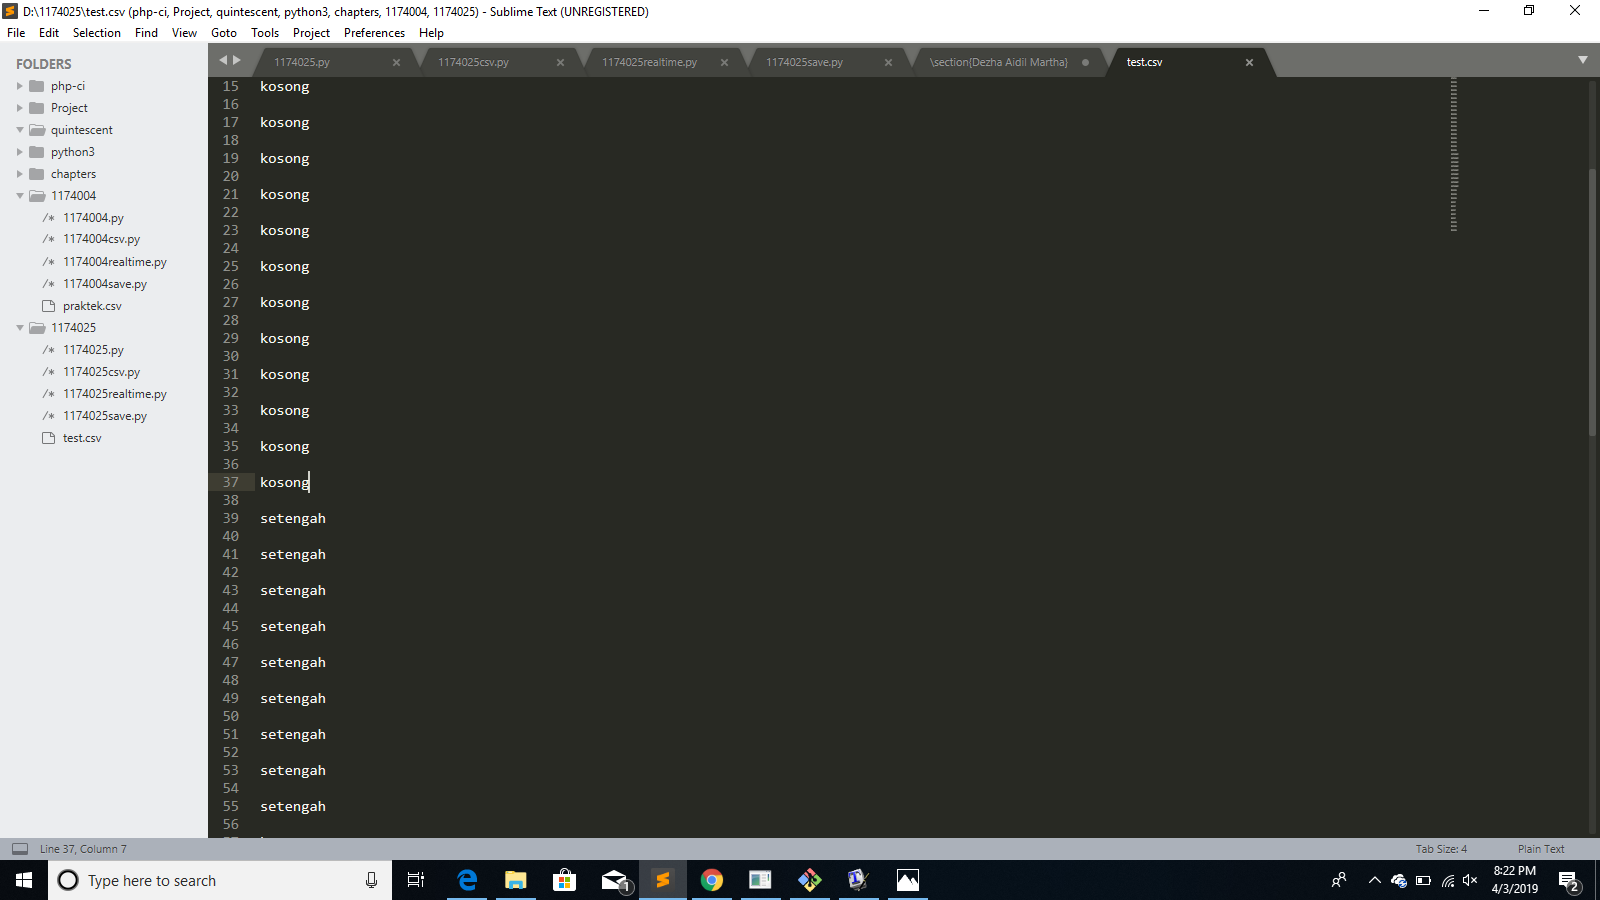
\includegraphics[scale=0.2]{figures/5/Praktek/1174025/csv.png}
	\centering
	\caption{Hasil dari pembacaan fungsi untuk mendapatkan data dari Arduino dan langsung ditulis kedalam file CSV.}
\end{figure}

\subsection{Soal No. 4}
Buatlah fungsi (file terpisah/library dengan nama NPMcsv.py) untuk membaca file csv hasil arduino dan mengembalikan ke fungsi!
\lstinputlisting[caption = Fungsi untuk membaca file CSV hasil Arduino dan mengembalikan fungsi., firstline=1, lastline=9]{src/5/Praktek/1174025/1174025csv.py}

\hfill \break
{\Large \textbf{Ketrampilan Penanganan Error}}

\subsection{Try Exception}
Tuliskan  peringatan  error  yang  didapat  dari  mengerjakan  praktek  kelima  ini, dan  jelaskan  cara  penanganan  error  tersebut.   dan  Buatlah  satu  fungsi  yang menggunakan try except untuk menanggulangi error tersebut.

\hfill \break
Peringatan error di praktek kelima ini, yaitu:
\begin{itemize}
	\item Syntax Errors
	Syntax Errors adalah suatu keadaan saat kode python mengalami kesalahan penulisan. Solusinya adalah memperbaiki penulisan kode yang salah terkadang kita bisa saja lupa dengan satu angka
		
	\item Type Error
	TypeError adalah exception yang akan terjadi apabila pada saat dilakukannya eksekusi terhadap suatu operasi atau fungsi dengan type object yang tidak sesuai. Solusi dari error ini adalah mengkoversi varibelnya sesuai dengan tipe data yang akan digunakan.
\end{itemize}

\hfill \break
Fungsi yang menggunakan try except untuk menanggulangi error.

\lstinputlisting[caption = Fungsi untuk menanggulangi error menggunakan Try Except., firstline=1, lastline=16]{src/5/Praktek/1174025/1174025.py}


\section{Evietania Charis Sujadi}
\subsection{Praktek}
\begin{enumerate}
\item Soal 1
\lstinputlisting[firstline=8, lastline=14]{src/5/Praktek/1174051/realtime_1174051.py}

\item Soal 2
\lstinputlisting[firstline=8, lastline=15]{src/5/Praktek/1174051/save_1174051.py}

\item Soal 3
\lstinputlisting[firstline=16, lastline=29]{src/5/Praktek/1174051/realtime_1174051.py}

\item Soal 4
\lstinputlisting[firstline=8, lastline=16]{src/5/Praktek/1174051/csv_1174051.py}

\end{enumerate}

\subsubsection{Penanganan Error}
cara untuk menangani eror yang dapat dilakukan adalah sebagai berikut:
\lstinputlisting[firstline=8, lastline=17]{src/5/Praktek/1174051/eror_1174051.py}





\bibliographystyle{IEEEtran}
%\def\bibfont{\normalsize}
\bibliography{references}


%%%%%%%%%%%%%%%
%%  The default LaTeX Index
%%  Don't need to add any commands before \begin{document}
\printindex

%%%% Making an index
%%
%% 1. Make index entries, don't leave any spaces so that they
%% will be sorted correctly.
%%
%% \index{term}
%% \index{term!subterm}
%% \index{term!subterm!subsubterm}
%%
%% 2. Run LaTeX several times to produce <filename>.idx
%%
%% 3. On command line, type  makeindx <filename> which
%% will produce <filename>.ind
%%
%% 4. Type \printindex to make the index appear in your book.
%%
%% 5. If you would like to edit <filename>.ind
%% you may do so. See docs.pdf for more information.
%%
%%%%%%%%%%%%%%%%%%%%%%%%%%%%%%

%%%%%%%%%%%%%% Making Multiple Indices %%%%%%%%%%%%%%%%
%% 1.
%% \usepackage{multind}
%% \makeindex{book}
%% \makeindex{authors}
%% \begin{document}
%%
%% 2.
%% % add index terms to your book, ie,
%% \index{book}{A term to go to the topic index}
%% \index{authors}{Put this author in the author index}
%%
%% \index{book}{Cows}
%% \index{book}{Cows!Jersey}
%% \index{book}{Cows!Jersey!Brown}
%%
%% \index{author}{Douglas Adams}
%% \index{author}{Boethius}
%% \index{author}{Mark Twain}
%%
%% 3. On command line type
%% makeindex topic
%% makeindex authors
%%
%% 4.
%% this is a Wiley command to make the indices print:
%% \multiprintindex{book}{Topic index}
%% \multiprintindex{authors}{Author index}

\end{document}

